\documentclass[11pt]{manual}
\usepackage[utf8]{inputenc}
\usepackage[footnotesep=15pt,foot=40pt]{geometry}                % See geometry.pdf to learn the layout options. There are lots.
\geometry{a4paper}                   % ... or a4paper or a5paper or ... 
%\geometry{landscape}                % Activate for for rotated page geometry
%\usepackage[parfill]{parskip}    % Activate to begin paragraphs with an empty line rather than an indent
\usepackage{graphicx}
\usepackage{listings}
\usepackage{color}
%\usepackage{amssymb}
\usepackage{makeidx}
\usepackage{url}
\usepackage{colortbl}
\usepackage[table]{xcolor}

\definecolor{seagreen}{RGB}{64,100,120}
\definecolor{darkpink}{RGB}{200,100,120}
\definecolor{light-gray}{gray}{0.85}
\definecolor{medium-gray}{gray}{0.5}
\usepackage[colorlinks=true,linkcolor=seagreen,citecolor=darkpink]{hyperref}

\newcommand{\idxconfflag}[1]{#1\index{Configuration macros!#1}\index{#1}}
\newcommand{\toreplace}[1]{$<$#1$>$}
\newcommand{\figcaption}[1]{\textit{\caption{\small #1}}}
\newcommand{\goil}{goil\index{goil, The oil compiler of Trampoline}}

\title{The Trampoline handbook}
\author{Jean-Luc B\'echennec, Florent Pavin}

\release{2.0}
\makeindex

\begin{document}
\maketitle
~\newpage
\setcounter{tocdepth}{2}
\tableofcontents

\part{The Real-Time Operating System}

%!TEX root = ./main.tex

\chapter{Tasks}
\label{chap:tasks}

\lettrine{A} task is an execution framework for the functions of the application\,\footnote{The term {\em Application} is also used in \autosar\ to designate a set of object, this manual uses OS Application to name the \autosar\ applications and Application to name the user level software.}. A task is a kind of \process. Tasks are executed concurrently and asynchronously, see \ref{sec:scheduling}. 2 kinds of task exist: basic tasks and extended tasks. A basic task cannot block (\ie\ it cannot use a service that may block) while an extended task can.
The tasks and their properties are declared in the OIL file, see \ref{oil:task}. Their functions are defined in a C file.

\section{States a task}
\label{sec:taskstate}

A task may be in different states. A basic task may be currently executing (in the \RUNNING\ state), ready to execute (in the \READY\ state) or not active at all (in the \SUSPENDED\ state). Figure \ref{fig:basictaskstates} shows the states of a basic task. An extended task has an additional \WAITING\ state.  Figure \ref{fig:extendedtaskstates} shows the states of an extended task. See section \ref{sec:internaltaskstate} for additional informations about the states of a task.

\begin{figure}[htbp] %  figure placement: here, top, bottom, or page
   \centering
   \parbox{.45\linewidth}{%
     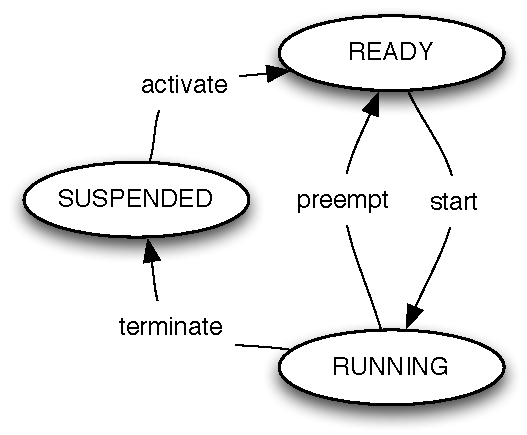
\includegraphics[scale=.6]{pictures/statesBasic.pdf} 
     \caption{States of a \BASIC\ task.}%
     \label{fig:basictaskstates}}%
%   \qquad
   \begin{minipage}{.55\linewidth}%
     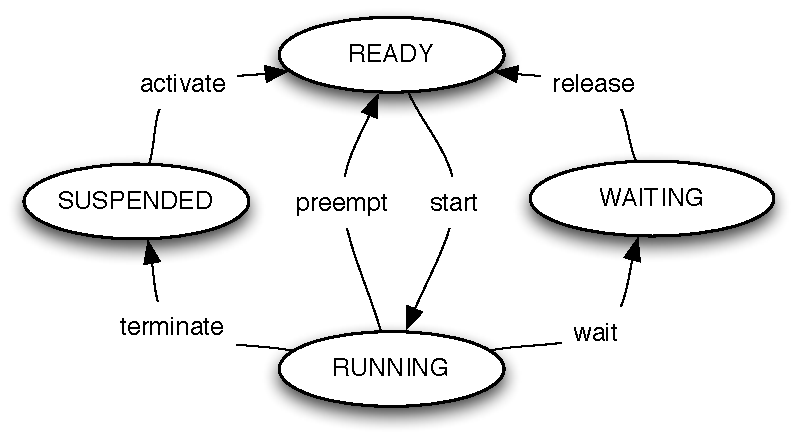
\includegraphics[scale=.6]{pictures/statesExtended.pdf} 
     \caption{States of an \EXTENDED\ task.}%
     \label{fig:extendedtaskstates}%
   \end{minipage}%
\end{figure} 


A task goes from one state to the other according to various conditions as shown in table \ref{tab:statetrans}.

\begin{table}[htbp]
\caption{Transition from state to state of a task.}
\rowcolors{1}{white}{light-gray}
\begin{longtable}[c]{l|l|l|p{7cm}}
\bf transition & \bf former state & \bf new state & \bf description\\
\hline
activate & \SUSPENDED & \READY & the task is set in the \READY\ state on one of the following occurrences: services \api{ActivateTask} or \api{ChainTask}, activation notification coming from an alarm, a schedule table or a message. \\
start & \READY & \RUNNING & the task is set to the running state and begin to execute because it has the highest priority in the system and has been elected by the scheduler. \\
terminate & \RUNNING & \SUSPENDED & the task is set to the \SUSPENDED\ state when it calls the \api{TerminateTask} or \api{ChainTask} service.\\
preempt & \RUNNING & \READY & the task is set to the \READY\ state when the scheduler starts a higher priority task.\\
wait & \RUNNING & \WAITING & the task may be set to the \WAITING\ state when it calls the service \api{WaitEvent}.\\
release & \WAITING & \READY & the task is set to the \READY\ state when it gets one of the  events it is waiting for. \\
\end{longtable}
\label{tab:statetrans}
\end{table}

\note{A system service may do more than one transition at a time. For instance, if a task is activated by calling \cfunction{ActivateTask} and its priority is higher than the priority of the current running task, the new task will go from \SUSPENDED\ to \RUNNING\ and the intermediate state \READY\ will not be observable.}

\section{The scheduling}
\label{sec:scheduling}

Trampoline schedules the tasks dynamically during the execution of the application. A task is scheduled according to its priority and whether it is preemptable or not. The priority of a task is given at design stage, and indicated in the OIL file using the \PRIORITY\ attribute, see \ref{sec:oiltask}, and may change during execution when the task gets or release a resource. The preemptability of a task may be set too. It is also indicated in the OIL file using the \SCHEDULE\ attribute, see \ref{sec:oiltask}.

A tasks continues to run until it is preempted because a task having a higher priority is put in the \READY\ state,  or it blocks because it is waiting for an event. Only extended tasks may block. If more than one task have the same priority, tasks are run one after the other because a task may not preempt an other task having the same priority. So there is no round robin among tasks of the same priority level.

A non-preemptable task runs until it calls \api{Schedule} and a higher priority task is in the \READY\ state or until it blocks. More informations about priority and preemptability may be found in chapter \ref{chap:resources}.

In the following examples, the horizontal axis is the time.  The state of the task is indicated in a rectangle that spans a period of time. When the task is running the rectangle is grayed. An up arrow \activate\ indicates a task activation and a down arrow \terminate\ a task termination.

\begin{figure}[htbp] %  figure placement: here, top, bottom, or page
   \centering
   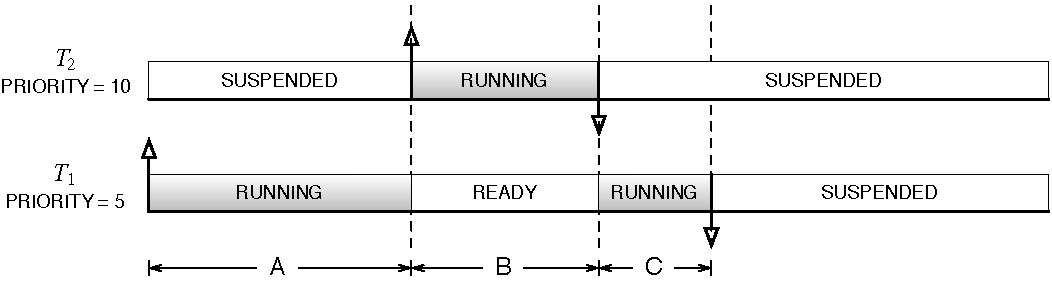
\includegraphics[scale=.7]{pictures/schedulingPreempt.pdf} 
   \caption{{\bfseries Scheduling of preemptable tasks.} During A period, $T_1$ is {\sffamily\scshape running} and $T_2$ is {\sffamily\scshape suspended}. Then $T_2$ is activated. Since $Prio(T_2) > Prio(T_1)$, $T_1$ is preempted and $T_2$ runs (B period). $T_2$ terminates and $T_1$ becomes {\sffamily\scshape running} again (C period) until it terminates.}
   \label{fig:schedulePreempt}
\end{figure} 

\begin{figure}[htbp] %  figure placement: here, top, bottom, or page
   \centering
   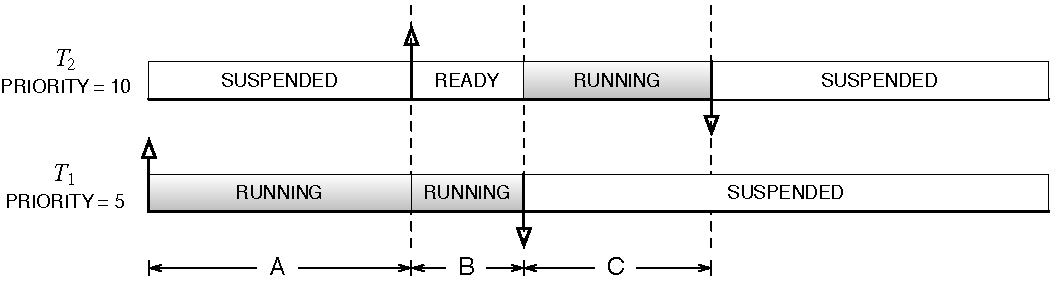
\includegraphics[scale=.7]{pictures/schedulingNonPreempt.pdf} 
   \caption{{\bfseries Scheduling of non-preemptable tasks.} During A period, $T_1$ is {\sffamily\scshape running} and $T_2$ is {\sffamily\scshape suspended}. Then $T_2$ is activated. Even if $Prio(T_2) > Prio(T_1)$, $T_1$ is non-preemptable and continues to run until it terminates (B period). In the meantime, $T_2$ is {\sffamily\scshape ready}. $T_1$ terminates and $T_2$ runs (C period) until it terminates.}
   \label{fig:schedulePreempt}
\end{figure} 

\section{Writing the code of a task}

Trampoline provides a \cmacro{TASK} macro to define a task in a C source file. The macro takes one argument which is the identifier of the task:

%\newpage
\begin{lstlisting}[language=C]
TASK(MyTask)
{
  /* code of the task */
  
  TerminateTask();
}
\end{lstlisting}

The code of the task is plain C.

The task should always end with a call to the \api{TerminateTask} service. See \ref{api:TerminateTask}.


\section{Tasks services}

\begin{service}{DeclareTask}{}

Each task has an identifier of type \ctype{TaskType}. This identifier is declared in the OIL file and is used in system calls to refer to a particular task. Before using such an identifier in your program, you have to declare it:

\begin{lstlisting}[language=C]
DeclareTask(MyTask);
\end{lstlisting}

This makes the \cdata{MyTask} identifier available in the current scope.

\note{ \servicename\ is a C macro. When the task has been define above using the macro \cmacro{TASK}, the identifier of the task is already in the scope and \cmacro{DeclareTask} is not needed.}

\argument{TaskType}{TaskID}{The id of the task to declare}
\end{service}

\begin{service}{ActivateTask}{StatusType}

\note{This service does a rescheduling}

Activates a new instance of a task. If activation counter has reached the maximum activation count or the task cannot be activated for timing protection purpose, the service fails. Otherwise if an instance is already active (\RUNNING\ or \READY), the state does not change and the activation is recorded to be done later. If no instance is active, the state of the task is changed to \READY.

Figures \ref{fig:scheduleT1lp}, \ref{fig:scheduleT1hp} and \ref{fig:scheduleMultiple} show 2 examples of task activation.

\argument{TaskType}{TaskID}{The id of the task to activate}
\resultcode{\OK}{No error, the task has been successfully activated}
\resultcodeext{\OSID}{Invalid TaskID. No task with such an id exists}
\resultcode{\OSLIMIT}{Too many activations of the task}
\end{service}

\begin{figure}[htbp] %  figure placement: here, top, bottom, or page
   \centering
   \begin{minipage}[c]{.6\linewidth}
   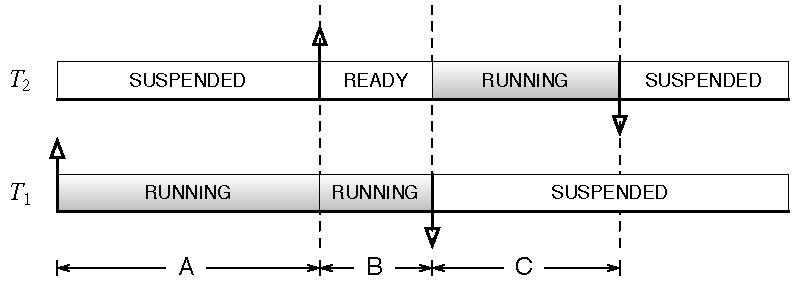
\includegraphics[scale=.7]{pictures/schedulingT1lp.pdf}
   \end{minipage}\hfill
   \begin{minipage}[c]{.3\linewidth}
   \begin{lstlisting}[language=C]
   TASK(T2) {
     ... /* C period */
     TerminateTask();
   }
   
   TASK(T1) {
     ... /* A period */
     ActivateTask(T2);
     ... /* B period */
     TerminateTask();
   }
 \end{lstlisting}
   \end{minipage}
   \caption{{\bfseries Activation of a lower priority task.} $Prio(T_1) \ge Prio(T_2)$. During A period, $T_1$ is {\sffamily\scshape running} and $T_2$ is {\sffamily\scshape suspended}. Then $T_1$ calls {\upshape\ttfamily ActivateTask(T2);}. Since $T_2$ does not have a higher priority, it becomes {\sffamily\scshape ready} (B period).  $T_1$ terminates and $T_2$ runs (C period) until it terminates.}
   \label{fig:scheduleT1lp}
\end{figure} 

\begin{figure}[htbp] %  figure placement: here, top, bottom, or page
   \centering
   \begin{minipage}[c]{.6\linewidth}
   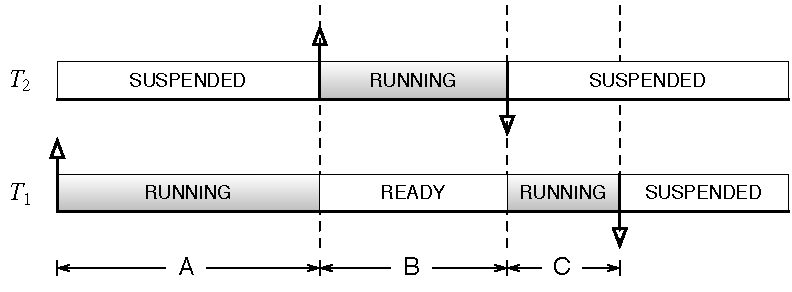
\includegraphics[scale=.7]{pictures/schedulingT1hp.pdf}
   \end{minipage}\hfill
   \begin{minipage}[c]{.3\linewidth}
   \begin{lstlisting}[language=C]
   TASK(T2) {
     ... /* B period */
     TerminateTask();
   }
   
   TASK(T1) {
     ... /* A period */
     ActivateTask(T2);
     ... /* C period */
     TerminateTask();
   }
 \end{lstlisting}
   \end{minipage}
   \caption{{\bfseries Activation of a higher priority task.} $Prio(T_1) < Prio(T_2)$. During A period, $T_1$ is {\sffamily\scshape running} and $T_2$ is {\sffamily\scshape suspended}. Then $T_1$ calls {\upshape\ttfamily ActivateTask(T2);}. Since $T_2$ has a higher priority, it becomes {\sffamily\scshape running} (B period).  $T_2$ terminates and $T_1$ resumes (C period) until it terminates.}
   \label{fig:scheduleT1hp}
\end{figure} 


\begin{figure}[htbp] %  figure placement: here, top, bottom, or page
   \centering
   \begin{minipage}[c]{.6\linewidth}
   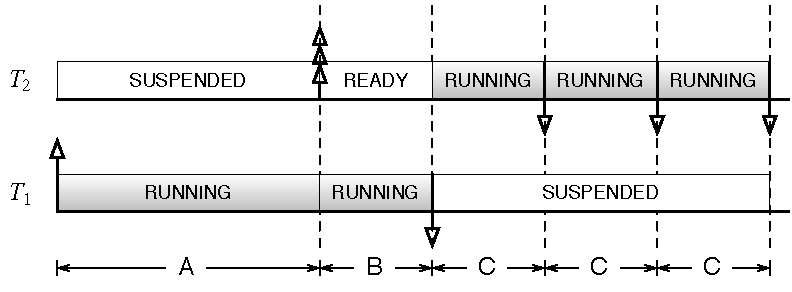
\includegraphics[scale=.7]{pictures/schedulingMultiple.pdf}
   \end{minipage}\hfill
   \begin{minipage}[c]{.3\linewidth}
   \begin{lstlisting}[language=C]
   TASK(T2) {
     ... /* C period */
     TerminateTask();
   }
   
   TASK(T1) {
     ... /* A period */
     ActivateTask(T2);
     ActivateTask(T2);
     ActivateTask(T2);
     ... /* B period */
     TerminateTask();
   }
 \end{lstlisting}
   \end{minipage}
   \caption{{\bfseries Multiple activations of a lower priority task.} $Prio(T_1) \ge Prio(T_2)$. During A period, $T_1$ is {\sffamily\scshape running} and $T_2$ is {\sffamily\scshape suspended}. Then $T_1$ calls {\upshape\ttfamily ActivateTask(T2);} 3 times. Since $T_1$ has a higher priority, $T_2$ does not run immediately and the 3 activations are recorded provided the ACTIVATION attribute in the OIL description of the task is a least 3 (B period). When $T_1$ terminates, the scheduler executes $T_2$ 3 times (C periods).}
   \label{fig:scheduleMultiple}
\end{figure} 



\begin{service}{ChainTask}{StatusType}

\note{This service does a rescheduling}

This service puts task TaskID in \READY\ state, and the calling task in the \SUSPENDED\ state. It acts as the \api{TerminateTask} service for the calling task.
\argument{TaskType}{TaskID}{The id of the task to activate}
\resultcode{\OK}{No error, the task TaskID has been successfully activated and the calling task has been successfully terminated. Note in this case {\ttfamily\servicename} does not return so actually \OK\ is never returned}
\resultcodeext{\OSID}{Invalid TaskID. No task with such an id exists}
\resultcode{\OSLIMIT}{Too many activations of the task}
\resultcodeext{\OSRESOURCE}{The calling task still held a resource}
\resultcodeext{\OSCALLLEVEL}{Called outside of a task}
\end{service}

\begin{figure}[htbp] %  figure placement: here, top, bottom, or page
   \centering
   \begin{minipage}[c]{.6\linewidth}
   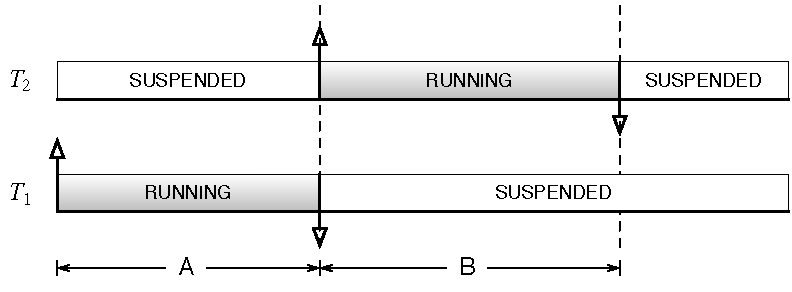
\includegraphics[scale=.7]{pictures/schedulingChain.pdf}
   \end{minipage}\hfill
   \begin{minipage}[c]{.3\linewidth}
   \begin{lstlisting}[language=C]
   TASK(T2) {
     ... /* B period */
     TerminateTask();
   }
   
   TASK(T1) {
     ... /* A period */
     ChainTask(T2);
   }
 \end{lstlisting}
   \end{minipage}
   \caption{{\bfseries Chaining of tasks.} During A period, $T_1$ is {\sffamily\scshape running} and $T_2$ is {\sffamily\scshape suspended}. Then $T_1$ calls {\upshape\ttfamily ChainTask(T2);}. $T_1$ terminates and $T_2$ is activated. Then $T_2$ runs (B periods).}
   \label{fig:scheduleMultiple}
\end{figure} 

\begin{service}{TerminateTask}{StatusType}

\note{This service does a rescheduling}

This service stops the calling task and puts it in \SUSPENDED\ state.
\resultcode{\OK}{No error, the calling task has been successfully terminated. Note in this case {\ttfamily\servicename} does not return so actually \OK\ is never returned}
\resultcodeext{\OSRESOURCE}{The calling task still held a resource}
\resultcodeext{\OSCALLLEVEL}{Called outside of a task}
\end{service}

\begin{service}{Schedule}{StatusType}
\note{This service does a rescheduling. 
Schedule does not deal directly with tasks but since it is a call to the scheduler, it is presented here.}

If called from a preemptable task that does not use an internal resource, Schedule has not effect. If called from a preemptable or a task that uses an internal resource, the priority of the task revert to its base priority and a rescheduling occurs.

Schedule allows to implement cooperative multitasking to insure synchronous rescheduling.
\resultcode{\OK}{No error.}
\resultcodeext{\OSRESOURCE}{The calling task still held a resource}
\resultcodeext{\OSCALLLEVEL}{Called outside of a task}
\end{service}

\begin{service}{GetTaskID}{StatusType}
\cfunction{\servicename} writes in the \var{TaskID} variable passed as reference the identifier of the task currently \RUNNING. If no task is currently \RUNNING\ because \cfunction{\servicename} was called from an ISR of before Trampoline is started, \constant{INVALID_TASK} is got.

\warning{The argument is a pointer. Do not pass an uninitialized pointer. Proper use of this service supposes a \ctype{TaskType} variable is instantiated, then its address is passed to \cfunction{\servicename} as shown in the example below:}

\begin{lstlisting}[language=C]
TaskType runningTaskID;
GetTaskID(&runningTaskID);
\end{lstlisting}

\resultcode{\OK}{No error.}
\resultcodeMP{\OSPROTECTIONMEMORY}{The caller does not have access to the addresses of \var{TaskID} reference} 
\argument{TaskRefType}{TaskID}{Reference to the task}
\end{service}

\begin{service}{GetTaskState}{StatusType}
\cfunction{\servicename} writes in the variable passed as reference in \var{State} the state of the task given in \var{TaskID}.

\warning{The \var{State} argument is a pointer. Do not pass an uninitialized pointer. Proper use of this service supposes a \ctype{TaskState} variable is instantiated, then its address is passed to \cfunction{\servicename} as shown in the example below:}

\begin{lstlisting}[language=C]
TaskStateType T1State;
GetTaskState(T1, &T1State);
\end{lstlisting}

\resultcode{\OK}{No error.}
\resultcodeext{\OSID}{Invalid TaskID. No task with such an id exists}
\resultcodeMP{\OSPROTECTIONMEMORY}{The caller does not have access to the addresses of \var{State} reference} 
\argument{TaskType}{TaskID}{The id of the task.}
\argument{TaskStateRefType}{State}{Reference to the state.}
\end{service}


%\strong{Processes} are both Tasks and ISRs category 2. Trampoline category 2 ISRs are like Basic Tasks except the priority level of the interrupt controller is raised to the priority of the ISR while the later is running.

\section{Inside Task management}
\label{sec:addtaskstate}

\subsection{Static attributes}

A task has the following static attributes:

\begin{description}
\item[The entry point of the task.] A pointer to the code of the task. When the scheduler start a task instance the first time, it uses this pointer to begin the execution.
\item[The internal resource] the task uses if any. An internal resource is automatically taken when a task enters the \RUNNING\ state and automatically released when the task leaves the \RUNNING\ state. See \ref{sec:internalresources} for more informations.
\item[The base priority] of the task as specified in the OIL file. This priority is used to reset the current priority when the task is activated.
\item[The maximum activation count] of the task as specified in the OIL file.
\item[The kind of task,] \BASIC\ or \EXTENDED.
\item[The task id.] Used for internal checking.
\item[The id of the OS Application] the tasks belong to (only available in \autosar\ \SC{3} and \SC{4}).
\item[The timing protection configuration] if any (only available in \autosar\ \SC{2} and \SC{4}).
\end{description}

\subsection{Dynamic attributes}

A task has also the following dynamic attributes:

\begin{description}
\item[The context.] This is the chunk of RAM where the current execution context of a task is stored when the task is in the \READY\ or \WAITING\ state. The execution context is the value of the microprocessor's registers (program counter, stack pointer, other working registers). So the context depends on the target on which Trampoline runs.
\item[The stack(s).] This is the chunk of RAM where registers are pushed for function call. This attributes depends on the target architecture. For instance, the C166 micro-controller uses 2 stacks.
\item[The current activation count.] When a task is activated while not in \SUSPENDED\ state, the activation is recorded and is actually done when the task returns to the \SUSPENDED\ state.  Many activation may be recorded according to the value given to the \oilattr{ACTIVATION} task OIL attribute. When a task is activated, the current activation count is compared to the maximum activation count and if $\ge$, the activation fails.
\item[The list of resources] the task currently owns.
\item[The current priority] of the task. This priority starts equal to the basic priority and may increase when the task get a resource.
\item[The state of the task] as defined in sections \ref{sec:taskstate} and \ref{sec:internaltaskstate}.
\item[The trusted counter.] If $=0$, the task is non-trusted. If $>0$ the task is trusted. See chapter \ref{chap:osapplications} for more informations. This counter is available if Trampoline is compiled with memory protection support.
\item[The activation allowed flag.] If true, the task may be activated. If false, it cannot be activated. This flag is set by the timing protection facility. It is available if Trampoline is compiled with timing protection support. See chapter \ref{chap:timingprotection}.
\end{description}

\subsection{Additional task states}
\label{sec:internaltaskstate}

In addition to states presented in section \ref{sec:taskstate}, 2 extra states are used for internal management: 

\begin{description}
\item[\AUTOSTART] This state is used to indicate what task should be started automatically when \api{StartOS} is called. An \AUTOSTART\ task is in this initial state but no task is in this state once the application code is running. \api{StartOS} iterates through the tasks and activates those that are in the \AUTOSTART\ state.
\item[\READYANDNEW] This state is used to flag a task that is ready but has its context uninitialized. This happens when the task has just been activated. The kernel initializes the context of the task the first time it goes to the \RUNNING\ state.
\end{description}

Figure \ref{fig:states} show a complete task state automaton for both basic and extended tasks with these states added.

\begin{figure}[htbp] %  figure placement: here, top, bottom, or page
   \centering
   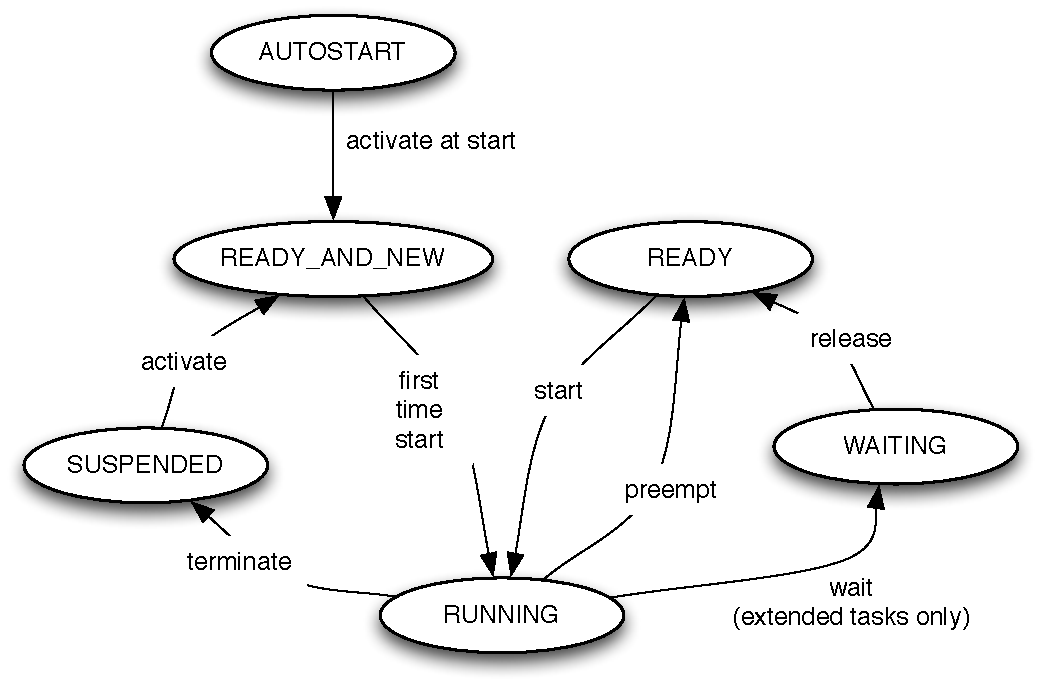
\includegraphics[width=4in]{pictures/states.pdf} 
   \caption{States of a task in Trampoline. \cmacro{AUTOSTART} is the initial state of autostart tasks. \cmacro{SUSPENDED} is the initial state of both non autostart tasks.}
   \label{fig:states}
\end{figure} 


\section{The {\em idle} task}

The {\em idle} task is activated by \api{StartOS}. It is a \BASIC\ task with a priority of 0 (\ie\ the lowest priority in the system, the lowest priority of tasks defined in the application is 1). So when no other task is currently running, the {\em idle} task run.

To be able to use specific platform capabilities (to put the micro-controller in stand by mode for example), this task calls repetitively a hardware specific function called \cfunction{tpl_sleep} (defined in \textit{machines/}). The tasks is then able to quantify the microprocessor occupation.

GOIL doesn't produce anything about this idle task (unlike application(s) task(s)). The idle task descriptor is defined in \file{tpl_os_kernel.c}.
%!TEX root = ./trampoline.tex

\chapter{Timing Protection Implementation}

The Timing Protection Implementation uses 2 timers. The first one is a {\em Free Running Timer} (FRT) which is used for {\em Time Frame}. The second one is a classical timer called {\em Timing Protection Timer} (TPT) which is used for \emph{Execution Time Budget}, \emph{Resource Locking Budget} and \emph{Interrupt Disabling Budget}.

\section{Low Level Functions}

These functions are provided by the {\em Board Support Package} and are used to manage the timers needed by the Timing Protection.

\subsection{FRT related functions}

\paragraph{\function{tpl_status tpl_start_frt(void)}} starts the FRT. On a microcontroller having a FRT that starts automatically when the system is powered on, this function does nothing but must be present since it is called by Trampoline in initialization stage. An error code is returned: {\em E\_OK} means no error, {\em E\_OS\_NOFUNC} means the FRT could not be started.

\paragraph{\function{tpl_status tpl_read_frt(tpl_tp_tick *out_value)}} write the current value of the FRT in \var{out_value}. An error code is returned: {\em E\_OK} means no error, {\em E\_OS\_NOFUNC} means the FRT could not be read.

\paragraph{\function{tpl_status tpl_elapsed_frt(tpl_tp_tick last_tick, tpl_tp_tick *out_value)}} write the number of ticks elapsed since \var{last_tick} in \var{out_value}. If the FRT has overflown/underflown between the time \var{last_tick} was get and the time \function{tpl_elapsed_frt} is called, \function{tpl_elapsed_frt} gives a correct value. An error code is returned: {\em E\_OK} means no error, {\em E\_OS\_NOFUNC} means the FRT could not be read.

\subsection{TPT related functions}

\paragraph{\function{tpl_status tpl_init_tpt(???)}} initializes the TPT. An error code is returned: {\em E\_OK} means no error, {\em E\_OS\_NOFUNC} means the TPT could not be initialized.

\paragraph{\function{tpl_status tpl_deinit_tpt(void)}} deinitializes the TPT. An error code is returned: {\em E\_OK} means no error, {\em E\_OS\_NOFUNC} means the TPT could not be deinitialized.

\paragraph{\function{tpl_status tpl_start_tpt(tpl_tp_tick delay)}} starts the TPT with an expiration delay equal to \var{delay} ticks. At that time, the \function{tpl_tpt_handler} function is called. An error code is returned: {\em E\_OK} means no error, {\em E\_OS\_NOFUNC} means the TPT could not be started because it is not initialized.

\paragraph{\function{tpl_status tpl_read_tpt(tpl_tp_tick *out_value)}} write the current value of the TPT in \var{out_value}. An error code is returned: {\em E\_OK} means no error, {\em E\_OS\_NOFUNC} means the TPT could not be read.

\paragraph{\function{tpl_status tpl_elapsed_tpt(tpl_tp_tick last_tick, tpl_tp_tick *out_value)}} write the number of ticks elapsed since \var{last_tick} in \var{out_value}. An error code is returned: {\em E\_OK} means no error, {\em E\_OS\_NOFUNC} means the TPT could not be read.

%!TEX root = ./trampoline.tex

\chapter{The communication library}

\section{Internals}


%!TEX root = ./main.tex

\chapter{System generation and compilation}

\lettrine{T}rampoline is a static operating system. This means all the objects (tasks, ISR, ...) are known at compile time. This way, an application is made of tasks' code and ISRs' code, application data, and statically initialized descriptor for each object the operating system manages. A system generation tool, like \goil, generates these descriptors in C files from an application configuration described in OIL or in XML. After that the Trampoline source code, the generated files and the application source code are compiled and linked together to produce an executable file as shown in figure \ref{fig:buildtrampoline}.

\begin{figure}[htbp] %  figure placement: here, top, bottom, or page
   \centering
   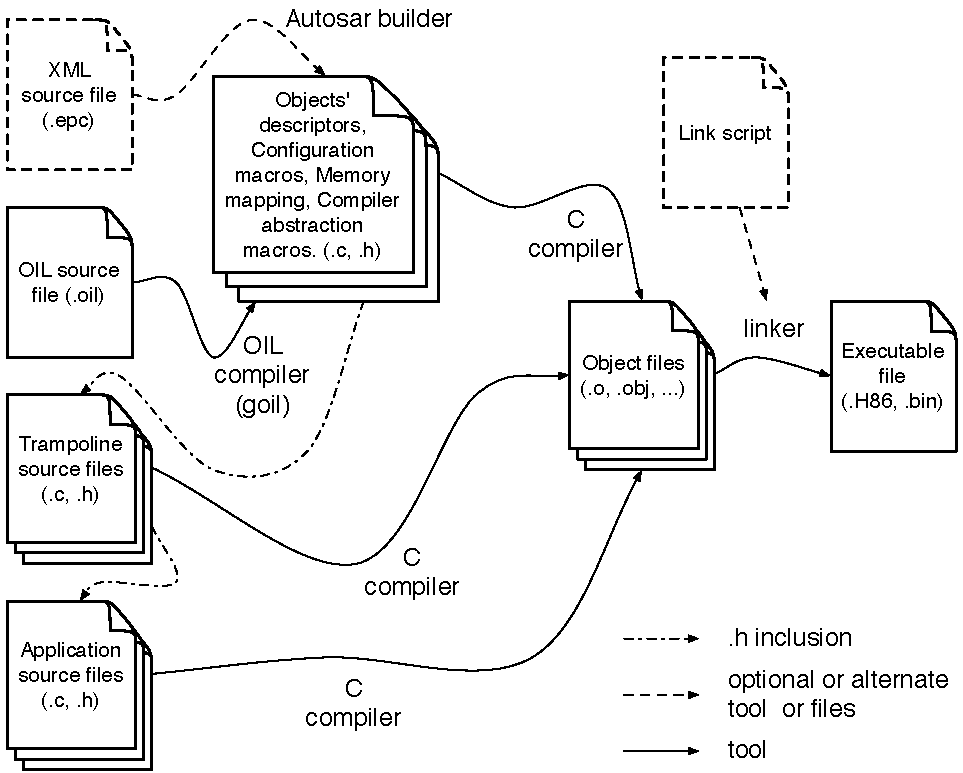
\includegraphics[width=4.3in]{pictures/buildProcess.pdf} 
   \caption{\textbf{Build process of an application with Trampoline.} Starting from the left, the .c and .h corresponding to the application description given in OIL (or XML) are generated by \goil\ (or another system generation tool, for instance an Autosar compliant one) and compiled using a C compiler. Trampoline source files are compiled too and include .h from the description for configuration purpose (see section \ref{sec:configmacros}). Application files are compiled and include .h files from Trampoline. All the object files are then linked together using an optional link script generated by \goil\ or provided with the application.}\label{fig:buildtrampoline}
\end{figure}

\section{The generated files}
\label{sec:generatedfiles}

The following files are generated by \goil\ from the OIL file or should be generated if you use a different system configuration tool. More information may be found in part \ref{part:goil}.

\rowcolors{1}{white}{light-gray}
\begin{longtable}[c]{l|p{4in}}
{\bf File name} & {\bf Usage} \\

\hline

tpl_app_define.h\index{tpl_app_define.h} & This file contains all the configuration macros (see section \ref{sec:configmacros}) and is included in all the Trampoline files to trigger conditional compilation. \goil\ generates this file using the \file{tpl_app_define_h.goilTemplate} template file.\\

tpl_app_config.h\index{tpl_app_config.h} & This file contains the declarations of the constants and functions required by the OSEK and Autosar standard (like OSMAXALLOWEDVALUE_x, OSTICKSPERBASE_x or OSMINCYCLE_x constants for counter x). \goil\ generates this file using the \file{tpl_app_config_h.goilTemplate} template file.\\

tpl_app_config.c\index{tpl_app_config.c} & This file contains the definitions of the constants and functions required by the OSEK and Autosar standard and the definitions of object descriptors used by Trampoline (see section \ref{sec:structs}) \goil\ generates this file using the \file{tpl_app_config_c.goilTemplate} template file.\\

tpl_app_custom_types.h\index{tpl_app_custom_types.h} & Some data types used by Trampoline are not statically defined. They are generated to fit size or performance criterions. For instance, the type used for a TaskType may be a byte if there is less than 256 tasks in the system and a word otherwise. This file defined these data types.\\

tpl_service_ids.h\index{tpl_service_ids.h} & This file is generated only if Trampoline is compiled with service calls implemented using a system call. It contains all the identifiers of the services used by the application according to the configuration. \goil\ generates this file using the \file{tpl_service_ids_h.goilTemplate} template file.\\

tpl_dispatch_table.c\index{tpl_dispatch_table.c} & This file is generated only if Trampoline is compiled with service calls implemented using a system call. It contains the dispatch table definition. See section \ref{sec:dispatchtable}. \goil\ generates this file using the \file{tpl_dispatch_table_c.goilTemplate} template file.\\

tpl_invoque.S\index{tpl_invoque.S} & This file is generated only if Trampoline is compiled with service calls implemented using a system call. It contains the API functions for system services. See section \ref{sec:invoque}. The extension (here .S) may change according to the assembler used. \goil\ generates this file using the \file{tpl_invoque.goilTemplate} and \file{service_call.goilTemplate} template files.\\

MemMap.h\index{MemMap.h} & This file is generated only if memory mapping is enabled. It contains macros for compiler abstraction memory mapping of functions and data as defined in the Autosar standard \cite{autosar31memorymapping}. \goil\ generates this file using the \file{MemMap_h.goilTemplate} template file.\\

Compiler.h\index{Compiler.h} & This file is generated only if memory mapping is enabled. It contains macros for the compiler abstraction of functions and pointer qualifier as defined in the Autosar standard \cite{autosar31compilerabstraction}. \goil\ generates this file using the \file{Compiler_h.goilTemplate} template file.\\

Compiler_Cfg.h\index{Compiler_Cfg.h} & This file is generated only if memory mapping is enabled. It contains macros for the compiler abstraction configuration as defined in the Autosar standard \cite{autosar31compilerabstraction}. \goil\ generates this file using the \file{Compiler_Cfg_h.goilTemplate} template file.\\

script.ld\index{script.ld} & This file is generated only if memory mapping is enabled. It contains a link script to map the executable in the target memory. \goil\ generates this file using the \file{script.goilTemplate} template file.\\

\end{longtable}

The following sections give details about the content of these files.

\section{The Configuration Macros}
\label{sec:configmacros}

Trampoline can be compiled with various options. These options are controlled by setting the appropriate preprocessor configuration macros%
\index{Configuration macros}.
These macros are usually set by \goil
using the template found in \file{tpl_app_define_h.goilTemplate} file to produce the \file{tpl_app_define.h}\index{tpl_app_define.h} file that is included by the files of Trampoline. However, a different generation tool may be used and it should comply to the specification presented in the following tables. When Trampoline is compiled, the coherency and consistency of the configuration macros are checked, by using the preprocessor macros located in the \file{tpl_config_check.h} file, to ensure they correspond to a supported configuration.

3 kinds of configuration macros are used: boolean macros, numerical macros, symbol macros and string macros. Boolean macros may take 2 values: \YES\ or \NO. All macros should be defined, Trampoline does not use the \lstinline[language=C]{#ifdef} or \lstinline[language=C]{\#ifndef} scheme to limit the occurrences of unwanted misconfigurations except to prevent multiple inclusions of the same header file.

\subsection{Number of objects macros}

These macros gives the number of objects of each kind (tasks, ISRs, resources, \ldots) and other values. They are used in Trampoline to check the validity of the various identifiers and to define tables of the corresponding size.
 
\rowcolors{1}{white}{light-gray}
\begin{longtable}[c]{l|l|p{3.5in}}
{\bf Macro}&{\bf Kind}&{\bf Effect}\\
\hline
\idxconfflag{PRIO_LEVEL_COUNT} &  Integer & The number of priority levels used in the system.\\
\idxconfflag{TASK_COUNT} & Integer & The number of tasks (basic and extended) used in the system.\\
\idxconfflag{EXTENDED_TASK_COUNT} & Integer & The number of extended tasks used in the system.\\
\idxconfflag{ISR_COUNT} & Integer & The number of ISR category 2 used in the system.\\
\idxconfflag{ALARM_COUNT} & Integer & The number of alarms used in the system.\\
\idxconfflag{RESOURCE_COUNT} & Integer & The number of resources used in the system.\\
\idxconfflag{SEND_MESSAGE_COUNT} & Integer & The number of send messages used in the system.\\
\idxconfflag{RECEIVE_MESSAGE_COUNT} & Integer & The number of receive messages used in the system.\\
\idxconfflag{SCHEDTABLE_COUNT} & Integer & The number of schedule tables used in the system. This macros is only used when \cmacro{WITH_AUTOSAR} is set to \YES.\\
\idxconfflag{COUNTER_COUNT} & Integer & The number of counters used in the system. This macros is only used when \cmacro{WITH_AUTOSAR} is set to \YES.\\
\idxconfflag{APP_COUNT} & Integer & The number of OS applications used in the system. This macros is only used when \cmacro{WITH_AUTOSAR} is set to \YES.\\
\idxconfflag{TRUSTED_FCT_COUNT} & Integer & The number of trusted functions used in the system. This macros is only used when \cmacro{WITH_AUTOSAR} is set to \YES.\\
\idxconfflag{RES_SCHEDULER_PRIORITY} & Integer & The priority of the \constant{RES_SCHEDULER} resource. This should be equal to the highest priority among the tasks.\\
\end{longtable}

\subsection{Error Handling Macros}
\label{sec:errorhook}

Error handling related macros are used to configure what kind of error Trampoline checks and what extra processing is done when an error is encountered.

\rowcolors{1}{white}{light-gray}
\begin{longtable}[c]{l|l|p{3.3in}}
{\bf Macro} & {\bf Kind} & {\bf Effect}\\
\hline
\idxconfflag{WITH_OS_EXTENDED} & Bool & When set to \YES, Trampoline system services perform error checking on their arguments. \cmacro{WITH_OS_EXTENDED} is set to \YES\ with a \oilattr{STATUS} = \constant{EXTENDED} and is set to \NO\ with a \oilattr{STATUS} = \constant{BASIC} in the OIL OS object.\\
\idxconfflag{WITH_ERROR_HOOK} & Bool & When set to \YES, the \cfunction{ErrorHook()} function is called if an error occurs. \cmacro{WITH_ERROR_HOOK} is set to \YES/\NO\ with a \cmacro{ERRORHOOK} = \TRUE/\FALSE\ in the OIL OS object.\\
\idxconfflag{WITH_USEGETSERVICEID} & Bool & When set to \YES, Trampoline system services store the id of the current service. This id may be retrieved in the \cfunction{ErrorHook()} function by using the \cfunction{OSErrorGetServiceId()} macro. \cmacro{WITH_USEGETSERVICEID} is set to \YES/\NO\ with a \oilattr{USEGETSERVICEID} = \TRUE/\FALSE\ in the OIL OS object.\\
\idxconfflag{WITH_USEPARAMETERACCESS} & Bool & When set to \YES, Trampoline system services store the arguments of the current service. These arguments may be retrieved in the \cfunction{ErrorHook()} function by using the ad-hoc access macros (see \cmacro{WITH_USEGETSERVICEID} above). \cmacro{WITH_USEPARAMETERACCESS} is set to \YES/\NO\ with a \oilattr{USEPARAMETERACCESS} = \TRUE/\FALSE\ in the OIL OS object.\\
\idxconfflag{WITH_COM_ERROR_HOOK} & Bool & When set to \YES, the communication error hook is called when error occurs in the communication sub-system. This macro is only available when \cmacro{WITH_COM} is set to \YES.\\
\idxconfflag{WITH_COM_USEGETSERVICEID} & Bool & When set to \YES, Trampoline/COM system services store the id of the current service. This id may be retrieved in the \cfunction{COMErrorHook()} function by using the \cfunction{COMErrorGetServiceId()} macro. \cmacro{WITH_COM_USEGETSERVICEID} is set to \YES/\NO\ with a \oilattr{COMUSEGETSERVICEID} = \TRUE/\FALSE\ in the OIL COM object.\\
\idxconfflag{WITH_COM_USEPARAMETERACCESS} & Bool & When set to \YES, Trampoline/COM system services store the arguments of the current service. These arguments may be retrieved in the \cfunction{COMErrorHook()} function by using the ad-hoc access macros (see \ref{sec:comerrorhook}). \cmacro{WITH_COM_USEPARAMETERACCESS} is set to \YES/\NO with a \oilattr{COMUSEPARAMETERACCESS} = \TRUE/\FALSE\ in the OIL COM object.\\
\idxconfflag{WITH_COM_EXTENDED} & Bool & When set to \YES, Trampoline/COM system services perform error checking on their arguments. \cmacro{WITH_COM_EXTENDED} is set to \YES\ with a \oilattr{COMSTATUS} = \EXTENDED\ and is set to \NO\ with a \oilattr{COMSTATUS} = \BASIC\ in the OIL COM object.\\
\end{longtable}

\subsection{Protection Macros}
\label{sec:protectionhook}

Protection macros deal with protection facilities provided by the \autosar\ standard.

\rowcolors{1}{white}{light-gray}
\begin{longtable}[c]{l|l|p{3.6in}}
{\bf Macro} & {\bf Kind} & {\bf Effect}\\
\hline
\idxconfflag{WITH_MEMORY_PROTECTION} & Bool & When set to \YES, Trampoline enables the memory protection facility. This is only supported on some ports (MPC5510 and ARM9 at time of writing). Memory protection requires the memory mapping and the use of system call. \cmacro{WITH_MEMORY_PROTECTION} is set to \YES/\NO\ with the \oilattr{MEMORY_PROTECTION} attribute of \oilattr{MEMMAP} object (see \ref{sec:memmap}) set to \TRUE/\FALSE.\\
\idxconfflag{WITH_TIMING_PROTECTION} & Bool & When set to \YES, Trampoline enables the timing protection facility. \cmacro{WITH_TIMING_PROTECTION} is set to \YES if the \oilattr{AUTOSAR_SC} is 2 or 4 (see \ref{sec:autosarsc}) and a least one of the objects specifies a timing protection related attribute in the OIL file.\\
\idxconfflag{WITH_PROTECTION_HOOK} &  Bool & When set to \YES, Trampoline calls the \cfunction{ProtectionHook()} with the appropriate argument when a protection fault occurs. \cmacro{WITH_PROTECTION_HOOK} is set to \YES with a \oilattr{PROTECTIONHOOK} = \TRUE in the OIL OS object.\\
\idxconfflag{WITH_STACK_MONITORING} & Bool & When set to \YES, Trampoline enables the stack monitoring. Each time a context switch occurs, the stack pointer is checked. If the stack pointer is outside the stack zone of the process, a fault occurs. \cmacro{WITH_STACK_MONITORING} is set to \YES with a \oilattr{STACKMONITORING} = TRUE in the oil OS object.\\
\end{longtable}

\subsection{Hook call macros}

Hook call macros control whether a hook is called or not.

\rowcolors{1}{white}{light-gray}
\begin{longtable}[c]{l|l|p{3.71in}}
{\bf Macro} & {\bf Kind} & {\bf Effect}\\
\hline
\idxconfflag{WITH_ERROR_HOOK} & Bool & see \ref{sec:errorhook}\\
\idxconfflag{WITH_PRE_TASK_HOOK} & Bool & When set to \YES, each time a task is scheduled, the function \cfunction{PreTaskHook()} is called. \cmacro{WITH_PRE_TASK_HOOK} is set to \YES/\NO\ with a \oilattr{PRETASKHOOK} = \TRUE/\FALSE\
  in the OIL OS object.\\
\idxconfflag{WITH_POST_TASK_HOOK} & Bool & When set to \YES, each time a task is descheduled, the function \cfunction{PostTaskHook()} is called. \cmacro{WITH_POST_TASK_HOOK} is set to \YES/\NO\ with a \oilattr{POSTTASKHOOK} = \TRUE/\FALSE\
  in the OIL OS object.\\
\idxconfflag{WITH_STARTUP_HOOK} & Bool & When set to \YES, the function \cfunction{StartupHook()} is called within the \api{StartOS} service.  \cmacro{WITH_STARTUP_HOOK} is set to \YES/\NO\ with a \oilattr{STARTUPHOOK} = \TRUE/\FALSE\ in the OIL OS object.\\
\idxconfflag{WITH_SHUTDOWN_HOOK} & Bool & When set to \YES, the function \cfunction{ShutdownHook()} is called within the \api{ShutdownOS} service. \cmacro{WITH_SHUTDOWN_HOOK} is set to \YES/\NO\ with a \oilattr{SHUTDOWNHOOK} = \TRUE/\FALSE\ in the OIL OS object.\\
\idxconfflag{WITH_PROTECTION_HOOK} & Bool & see \ref{sec:protectionhook}\\
\end{longtable}

\subsection{Miscellaneous macros}

Here are the other available macros:

\rowcolors{1}{white}{light-gray}
\begin{longtable}[c]{l|l|p{3.25in}}
{\bf Macro} & {\bf Kind} & {\bf Effect}\\
\hline
\idxconfflag{WITH_USERESSCHEDULER} & Bool & When set to \YES, the \constant{RES_SCHEDULER} resource is used by at least one process. \cmacro{WITH_USERESSCHEDULER} is set to \YES/\NO\ with a \oilattr{USERESSCHEDULER} = \TRUE/\FALSE\ in the OIL OS object.\\
\idxconfflag{WITH_SYSTEM_CALL} & Bool & When set to \YES, services are called by the mean of a system call, also known as a software interrupt (see section \ref{sec:systemcall}). \cmacro{WITH_SYSTEM_CALL} is set to \YES/\NO\ according to the target architecture and requires a memory mapping\\
\idxconfflag{WITH_MEMMAP} & Bool & When set to \YES, a memory mapping is used. A \file{MemMap.h} files giving the available memory segments is included and should be generated or provided by the user. \goil\ generates such a file.
  \cmacro{WITH_MEMMAP} is set to \YES/\NO\ with a \oilattr{MEMMAP} = \TRUE/\FALSE\ in the OIL OS object.\\
\idxconfflag{WITH_COMPILER_SETTINGS} & Bool & When set to \YES, the compiler dependent macros are used. \file{Compiler.h} and \file {Compiler_Cfg.h} files are includes and should be generated or provided by the user. \goil\ generates these  files if \oilattr{MEMMAP} is \TRUE\ and the \oilattr{COMPILER} sub-attribute is set.\\
\idxconfflag{WITH_AUTOSAR} & Bool & When set to \YES, Trampoline contains additional system services, code and declarations related to the \autosar\ standard. For instance, the counter descriptor includes the counter type (hardware or software).   \cmacro{WITH_AUTOSAR} is set to \YES/\NO\ when at least one \autosar\ object is present in the system configuration (OIL file for instance).\\
\idxconfflag{TRAMPOLINE_BASE_PATH} & String & The path to Trampoline root directory.\\
\idxconfflag{AUTOSAR_SC} & Integer & The \autosar\ scalability class\index{Scalability class} ranging from 0 to 4. 0 means OSEK\\
\idxconfflag{WITH_OSAPPLICATION} & Bool & When set to \YES, OS Application\index{OS Application} are used.\\
\idxconfflag{WITH_TRACE} & Bool & When set to \YES, the tracing of the operating system is enabled.\\
\idxconfflag{TRACE_TASK} & Bool & When set to \YES, task (de)scheduling events are traced. Only available if \cmacro{WITH_TRACE} is set to \YES.\\
\idxconfflag{TRACE_ISR} & Bool & When set to \YES, ISR category 2 (de)scheduling events are traced. Only available if \cmacro{WITH_TRACE} is set to \YES.\\
\idxconfflag{TRACE_RES} & Bool & When set to \YES, resources get and release are traced. Only available if \cmacro{WITH_TRACE} is set to \YES.\\
\idxconfflag{TRACE_ALARM} & Bool & When set to \YES, alarm activities are traced. Only available if \cmacro{WITH_TRACE} is set to \YES.\\
\idxconfflag{TRACE_U_EVENT} & Bool & When set to \YES, user events are traced. Only available if \cmacro{WITH_TRACE} is set to \YES.\\
\idxconfflag{TRACE_FORMAT} & Symbol & Trace format. A function named \cfunction{tpl_trace_format_\toreplace{\cmacro{TRACE_FORMAT}}} is expected. Only available if \cmacro{WITH_TRACE} is set to \YES.\\
\idxconfflag{TRACE_FILE} & String & File name where the trace is stored. Usable on Posix target only. Only available if \cmacro{WITH_TRACE} is set to \YES.\\
\idxconfflag{WITH_IT_TABLE} & Bool & When set to \YES, the external interrupts are dispatched using a table of fonction pointers.\\
\idxconfflag{WITH_COM} & Bool & When set to \YES, internal communication is used.\\
\idxconfflag{TPL_COMTIMEBASE} & Integer & The \oilattr{COMTIMEBASE} expressed in nanoseconds.\\
\idxconfflag{WITH_COM_STARTCOMEXTENSION} & Bool & When set to \YES, the communication extension function is called.\\
\end{longtable}

\section{Application configuration}

The application configuration is generated by \goil\ using the template found in \file{tpl_app_config_h.goilTemplate} file and \file{tpl_app_config_c.goilTemplate} file to produce the \file{tpl_app_define.h}\index{tpl_app_define.h} and \file{tpl_app_define.c}\index{tpl_app_define.c} files.

\subsection{Counter related constants declaration}

The \file{tpl_app_config.h} files contains the counters related constants: those of the SystemCounter\footnote{the default counter of an OSEK operating system} and those of the counters defined by the user. The SystemCounter constants are located in the generated files because the SystemCounter default attributes may be modified by the user in the OIL or XML file. The constants of a user defined counter are declared as follow:

\begin{lstlisting}[language=C]
extern CONST(tpl_tick, OS_CONST) OSTICKSPERBASE_<counter name>;
extern CONST(tpl_tick, OS_CONST) OSMAXALLOWEDVALUE_<counter name>;
extern CONST(tpl_tick, OS_CONST) OSMINCYCLE_<counter name>;
\end{lstlisting}

Where \toreplace{counter name} is obviously the name given to the counter in the confguration. For the SystemCounter, the following constants are declared:

%\begin{lstlisting}[language=C]
%extern CONST(tpl_tick, OS_CONST) OSTICKSPERBASE;
%extern CONST(tpl_tick, OS_CONST) OSMAXALLOWEDVALUE;
%extern CONST(tpl_tick, OS_CONST) OSMINCYCLE;
%\end{lstlisting}

\subsection{Events definition}

The \file{tpl_app_config.c} file should contain the event mask definitions. For each event defined in the configuration, the following lines should appear:

\begin{lstlisting}[language=C]
#define API_START_SEC_CONST_UNSPECIFIED
#include "tpl_memmap.h"

#define <event name>_mask <mask value>
CONST(EventMaskType, AUTOMATIC) <event name> = <event name>_mask;

#define API_STOP_SEC_CONST_UNSPECIFIED
#include "tpl_memmap.h"
\end{lstlisting}

Where \toreplace{event name} is the name given to the event in the configuration and \toreplace{mask value} is the value set by the user in the configuration or, when set to AUTO, the value computed by the generation tool.

\subsection{Standard resources definition}

Standard resources need the definition of an identifier used to reference the resource in a system service (\cfunction{GetResource()} and \cfunction{ReleaseResource()}) and an instance of a \ctype{tpl_resource} structure (see \ref{sec:structtplresource}). This is done with the following definitions:

\begin{lstlisting}[language=C]
#define API_START_SEC_CONST_UNSPECIFIED
#include "tpl_memmap.h"

#define <resource name>_id <resource id>
CONST(ResourceType, AUTOMATIC) <resource name> = <resource name>_id;

#define API_STOP_SEC_CONST_UNSPECIFIED
#include "tpl_memmap.h"

#define OS_START_SEC_VAR_UNSPECIFIED
#include "tpl_memmap.h"

VAR(tpl_resource, OS_VAR) <resource name>_rez_desc = {
  /* ceiling priority of the resource */  <resource priority>,
  /* owner previous priority          */  0,
  /* owner of the resource            */  INVALID_PROC_ID,
#if WITH_OSAPPLICATION == YES
  /* OS Application id                */  <resource application id>,
#endif    
  /* next resource in the list        */  NULL
};

#define OS_STOP_SEC_VAR_UNSPECIFIED
#include "tpl_memmap.h"
\end{lstlisting}

Where \toreplace{resource name} is the name given to the resource in the configuration, \toreplace{resource priority} is the priority of the resource that is computed by the generation tool and is the maximum priority of the processes that use the resource and \toreplace{resource application id} is the identifier of the OS Application the resource belongs to. Since this field is protected by \var{WITH_OSAPPLICATION}, it may be leaved empty when no OS Application is used.

\toreplace{resource id} ranges from 0 to the number of standard resources minus 1. Once every standard resource descriptor is defined, a table gathering pointers to the resource descriptors and indexed by the resource id has to be defined. This table is used by system services to get the resource descriptor from the resource id. Suppose 3 standard resource, \var{motor1}, \var{motor2} and \var{dac} has been defined and RES_SCHEDULER is used, the table should be as follow:

\begin{lstlisting}[language=C]
#define OS_START_SEC_CONST_UNSPECIFIED
#include "tpl_memmap.h"
CONSTP2VAR(tpl_resource, AUTOMATIC, OS_APPL_DATA)
tpl_resource_table[RESOURCE_COUNT] = {
  &motor1_rez_desc,
  &motor2_rez_desc,
  &dac_rez_desc,
  &res_sched_rez_desc  
};
#define OS_STOP_SEC_CONST_UNSPECIFIED
#include "tpl_memmap.h"
\end{lstlisting}

\var{\&res_sched_rez_desc}, the pointer to the resource descriptor of RES_SCHEDULER should always be the last element of the table. If RES_SCHEDULER is not used, simply remove it from the table.

\subsection{Tasks definition}

Each task needs an identifier to reference a task un a system service (\cfunction{ActivateTask()}, \cfunction{ChainTask()}, \cfunction{GetTaskState()}, \cfunction{SetEvent()} and \cfunction{GetEvent()}) and the declaration of the task function. The following definitions should appear for each task:

\begin{lstlisting}[language=C]
#define API_START_SEC_CONST_UNSPECIFIED
#include "tpl_memmap.h"

#define <task name>_id <task id>
CONST(TaskType, AUTOMATIC) <task name> = <task name>_id;

#define API_STOP_SEC_CONST_UNSPECIFIED
#include "tpl_memmap.h"

#define APP_Task_<task name>_START_SEC_CODE
#include "tpl_memmap.h"

FUNC(void, OS_APPL_CODE) <task name>_function(void);

#define APP_Task_<task name>_STOP_SEC_CODE
#include "tpl_memmap.h"
\end{lstlisting}

Where \toreplace{task name} is the name given to the task in the configuration and \toreplace{task id} is the identifier of the task computed by the system generation tool. Task ids should range from 0 to the number of tasks minus 1. In addition, id allocation must start with extended tasks first and basic task after. In addition an instance of the static task descriptor must be provided:

\begin{lstlisting}[language=C]
#define OS_START_SEC_CONST_UNSPECIFIED
#include "tpl_memmap.h"
CONST(tpl_proc_static, OS_CONST) <task name>_task_stat_desc = {
  /* context                  */  <task name>_CONTEXT,
  /* stack                    */  <task name>_STACK,
  /* entry point (function)   */  <task name>_function,
  /* internal ressource       */  <internal resource>,
  /* task id                  */  <task name>_id,
#if WITH_OSAPPLICATION == YES
  /* OS application id        */  <application>,
#endif
  /* task base priority       */  <task priority>,
  /* max activation count     */  <task activation>,
  /* task type                */  <task type>
#if WITH_AUTOSAR_TIMING_PROTECTION == YES
  /* pointer to the timing
     protection descriptor    */  ,<timing protection>
#endif
};
#define OS_STOP_SEC_CONST_UNSPECIFIED
#include "tpl_memmap.h"
\end{lstlisting}

Where \toreplace{task name} is the name given to the task in the configuration. \toreplace{internal resource} mays be one of the following:

\begin{itemize}
\item a pointer to the internal resource descriptor (see \ref{sec:internalresource}) if an internal resource has been defined in the configuration;
\item a pointer to the scheduler internal resource if the task has been defined as non-preemptable in the configuration;
\item NULL if none of the above cases apply.
\end{itemize}

\toreplace{application} is the id of the OS Application the task belongs to when OS Application are used or, when they are not used, nothing at all. \toreplace{task priority} is the priority of the task as computed by the \sysgen. \toreplace{task activation} is the maximum number of task activation allowed as defined in the configuration. \toreplace{task type} may be \EXTENDED\ or \BASIC. \toreplace{timing protection} is a pointer to the timing protection descriptor or NULL if no timing protection is defined for the task.

Also an instance of the dynamic task descriptor must be provided:

\begin{lstlisting}[language=C]
#define OS_START_SEC_VAR_UNSPECIFIED
#include "tpl_memmap.h"

VAR(tpl_proc, OS_VAR) <task name>_task_desc = {
  /* resources                      */  NULL,
#if WITH_MEMORY_PROTECTION == YES
  /* if > 0 the process is trusted  */  <trusted count>,    
#endif /* WITH_MEMORY_PROTECTION */
  /* activate count                 */  0,
  /* task priority                  */  <task priority>,
  /* task state                     */  <task state>
#if WITH_AUTOSAR_TIMING_PROTECTION == YES
  /* activation allowed             */  ,TRUE
#endif
};

#define OS_STOP_SEC_VAR_UNSPECIFIED
#include "tpl_memmap.h"
\end{lstlisting}

Where \toreplace{task name} is the name given to the task in the configuration. \toreplace{trusted count} is 0 if the task belongs to a non trusted OS Application and 1 if the tasks belongs to a trusted OS Application. \toreplace{task priority} is the priority of the task as computed by the \sysgen. \toreplace{task state} is the initial state of the task and must be set to AUTOSTART or SUSPENDED.

If the task is an EXTENDED one, an event mask descriptor is added:

%\lstdefinelanguage[trampconf]{C}{morecomment=[s][\color{red}]{<}{>}}

\begin{lstlisting}[language=C]
VAR(tpl_task_events, OS_VAR) <task name>_task_evts = {
  /* event set  */ 0,
  /* event wait */ 0
};
\end{lstlisting}

Where \toreplace{task name} is the name given to the task in the configuration.


%!TEX root = ./main.tex

\chapter{Ports details}

\section{PowerPC}

\subsection{System services} \label{sec:systemservices}

The PowerPC port uses the \asfct{sc} software interrupt to call system services \cite{mpc32bsc}. \asfct{sc} stands for System Call. It saves the current \reg{PC} in \reg{SRR0} register and the current \reg{MSR} in \reg{SRR1} register and jump to the System Call handler.

The id of the system service to call is given in the \reg{r0} register and \reg{r0} save and restore are added around. For instance, the following listing gives the \api{ActivateTask} service code. These function are generated from templates by goil (see \ref{sec:generatedfiles}) and are part of the {\em invoque} layer (see \ref{sec:invoque}):

\begin{lstlisting}[language=C]
  .global ActivateTask
ActivateTask:
  subi r1,r1,4                       /* make room on stack    */
  stw  r0,0(r1)                      /* save r0               */
  li   r0,OSServiceId_ActivateTask   /* load r0 with the id   */
  sc                                 /* system call           */
  lwz  r0,0(r1)                      /* restore r0            */
  addi r1,r1,4                       /* restore stack         */
  blr                                /* return                */
  
  .type ActivateTask,@function
  .size ActivateTask,$$-ActivateTask
\end{lstlisting}

When the System Call begin execution, the process stack has the mapping depicted in figure \ref{fig:stackbeginningSC}.

\begin{figure}[htbp] %  figure placement: here, top, bottom, or page
\begin{minipage}{0.5\textwidth}
    \centering
  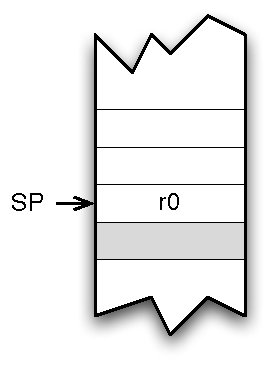
\includegraphics[scale=.6]{pictures/PStackAfterInvoque} 
\end{minipage}
\begin{minipage}{0.5\textwidth}
   \caption{Process stack mapping at the beginning of the System Call handler. The grayed zone represents an unknown content depending on from where the service was called.}\label{fig:stackbeginningSC}
\end{minipage}
\end{figure}

\subsection{Dispatching the service call}

The System Call handler is usually located in the \hex{0C00} exception handler but, depending on the CPU kind, it may be located elsewhere. Since the available memory for the interrupt or exception handler may vary, a jump is made to the \cfunction{tpl_sc_handler}.%:

%\begin{lstlisting}
%  .section  .SC_vector  CODE_ACCESS_RIGHT
%tpl_sc_vector:
%  b   tpl_sc_handler
%
%  .section  .SC_handler CODE_ACCESS_RIGHT
%\end{lstlisting}

\cfunction{tpl_sc_handler} performs the following tasks:
\begin{penum}
\item saves additional registers to be able to work
\item disables memory protection
\item switches to kernel stack if needed
\item calls the service
\item performs a context switch if needed and programs the MPU.
\item switches back to the process stack if needed
\item enable memory protection
\item restore registers
\item get back to the process
\end{penum}

\note{Currently the PowerPC port does not support tasks that use floating point registers}

\subsubsection{Saving additional registers}

The following registers are saved: \var{lr}, \var{cr}, \var{r11} and \var{r12}. In fact, it should be not necessary to save \var{r11} and \var{r12} because these registers are volatile as defined in the PowerPC EABI \cite{PPCeabi} but we prefer a conservative approach. Register saving is done by the following code at start of the \cfunction{tpl_sc_handler} and the mapping of the process stack is depicted at figure \ref{fig:stackSavingSC}:

\begin{lstlisting}[language=C]
  subi  r1,r1,PS_FOOTPRINT  /* Make room on stack */

  stw   r11,PS_R11(r1)      /* Save r11           */
  stw   r12,PS_R12(r1)      /* Save r12           */
  mflr  r11
  stw   r11,PS_LR(r1)       /* Save lr            */
  mfcr  r11
  stw   r11,PS_CR(r1)       /* Save cr            */
\end{lstlisting}

\begin{figure}[htbp] %  figure placement: here, top, bottom, or page
\begin{minipage}{0.5\textwidth}
    \centering
  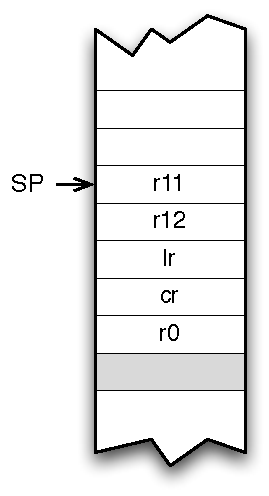
\includegraphics[scale=.6]{pictures/PStackAfterSCSaving} 
\end{minipage}
\begin{minipage}{0.5\textwidth}
   \caption{Process stack mapping after additional registers have been saved by the beginning of the System Call handler.}\label{fig:stackSavingSC}
\end{minipage}
\end{figure}

\subsubsection{Disabling memory protection}

This part of the dispatch layer is done in the \cfunction{tpl_enter_kernel} function and is assembled only if \cmacro{WITH_MEMORY_PROTECTION} is set to \YES. After saving the \reg{lr}, the \cfunction{tpl_kernel_mp} function is called and does the actual job. At last \reg{lr} is restored.

\begin{lstlisting}[language=C]
#if WITH_MEMORY_PROTECTION == YES
  /*
   * Switch to kernel mem protection scheme
   */
  subi  r1,r1,4
  mflr  r11
  stw   r11,0(r1)       /* save lr on the current stack */
  bl    tpl_kernel_mp   /* disable memory protection    */
  lwz   r11,0(r1)       /* restore lr                   */
  mtlr  r11
  addi  r1,r1,4
#endif
\end{lstlisting}

\subsubsection{Switching to the kernel stack}

Once the dispatch layer has saved the registers it uses and has switched to the kernel memory protection scheme, it switches to the kernel stack. However the kernel stack could used already because a call to a \cfunction{PreTaskHook} or a \cfunction{PostTaskHook} is done on the kernel stack and such a hook may call a service. So the dispatch layer is reentrant. The number of reentrant calls is counted by the \var{tpl_reentrancy_counter}. In addition the process stack pointer (\reg{r1}), \reg{SRR0} and \reg{SRR1} are saved in the kernel stack. The kernel stack mapping is shown in figure \ref{fig:kernelstackmapping}. For a reentrant call, the same frame is build over the current one. The switch to the kernel stack is done as follow:

\begin{lstlisting}[language=C]
  /*
   * Check the reentrency counter value and increment it
   * if the value is 0 before the inc, then we switch to
   * the system stack.
   */
  lis   r11,TPL_HIG(tpl_reentrancy_counter)
  ori   r11,r11,TPL_LOW(tpl_reentrancy_counter)
  lwz   r12,0(r11)    /* get the value of the counter */
  cmpwi r12,0
  addi  r12,r12,1
  stw   r12,0(r11)
  bne   no_stack_change
  
  /*
   * Switch to the kernel stack
   *
   * Get the pointer to the bottom of the stack
   */  
  lis   r11,TPL_HIG(tpl_kernel_stack_bottom)
  ori   r11,r11,TPL_LOW(tpl_kernel_stack_bottom)
  stw   r1,KS_SP-KS_FOOTPRINT(r11)  /* save the sp of the caller */
  mr    r1,r11                      /* set the kernel stack      */
  
no_stack_change:
  /*
   * make space on the stack to call C functions
   */
  subi  r1,r1,KS_FOOTPRINT
\end{lstlisting}

\begin{figure}[htbp] %  figure placement: here, top, bottom, or page
\begin{minipage}{0.5\textwidth}
    \centering
  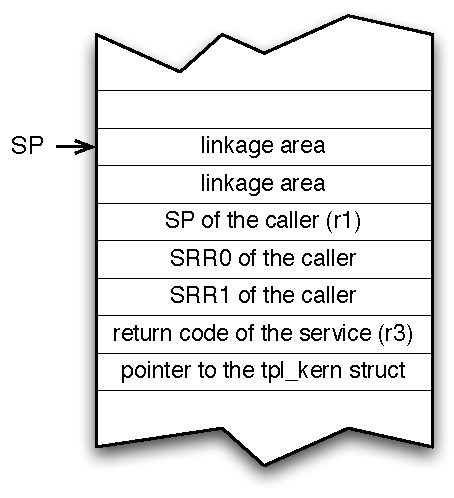
\includegraphics[scale=.6]{pictures/KStackMapping} 
\end{minipage}
\begin{minipage}{0.5\textwidth}
  \caption{Kernel stack mapping after allocation.}\label{fig:kernelstackmapping}
\end{minipage}
\end{figure}

\subsubsection{Calling the service}

Since the registers used to pass parameters to a function, that is \reg{r3} to \reg{r10} as documented in \cite{PPCeabi}, have not been changed until now, calling the function that implements the service respects the register usage conventions.

The first thing to do is to get the function pointer corresponding to the service id. The service id is in \reg{r0} as explained in \ref{sec:systemservices} and is used as an index to the \var{tpl_dispatch_table}.

\begin{lstlisting}[language=C]
  slwi  r0,r0,2                           /* compute the offset    */
  /*
   * load the ptr to the dispatch table
   */
  lis   r11,TPL_HIG(tpl_dispatch_table)     
  ori   r11,r11,TPL_LOW(tpl_dispatch_table)
  lwzx  r11,r11,r0                  /* get the ptr to the service  */
  mtlr  r11                         /* put it in lr for future use */
\end{lstlisting}

The second thing to do is to reset the \var{tpl_need_switch} flag that triggers a context switch. This flag (a byte) is located in the \var{tpl_kern} kernel struct. This is done as follow:

\begin{lstlisting}[language=C]
  lis   r11,TPL_HIG(tpl_kern)
  ori   r11,r11,TPL_LOW(tpl_kern)
  stw   r11,KS_KERN_PTR(r1)        /* save the ptr for future use  */
  li    r0,NO_NEED_SWITCH
  stb   r0,20(r11)
\end{lstlisting}

In the future \var{tpl_kern} will be reused, so its address is saved in the kernel stack.

Then, to allow reentrancy for a service call in a hook, the \reg{RI} bit of the \reg{MSR} is set to 1. Without that, a \asfct{sc} cannot be  properly executed.

\begin{lstlisting}[language=C]
  mfmsr r11
  ori   r11,r11,RI_BIT_1
  mtmsr r11
\end{lstlisting}

At last, the service is called:

\begin{lstlisting}[language=C]
  blrl
\end{lstlisting}

\subsubsection{Context switch}

The \var{tpl_need_switch} flag that as been possibly modified by the service is now checked to do a context switch if needed.

\begin{lstlisting}[language=C]
  lwz   r11,KS_KERN_PTR(r1) /* get back the tpl_kern address */
  lbz   r12,20(r11)         /* get the tpl_need_switch flag  */
  andi. r0,r12,NEED_SWITCH  /* check if a switch is needed   */
  beq   no_context_switch
\end{lstlisting}

A context switch is performed in 3 steps. The first one is the context save of the process that loses the CPU. This step is optional because if the service was a \api{TerminateTask} or a \api{ChainTask}, the context needs not to be saved. This information is in the \var{tpl_need_switch} flag. Before doing the actual context save, the return value of the service must be saved in the proper location of the kernel stack. The \cfunction{tpl_save_context} function will read it from this location and expects a pointer to the context saving area or the process in \reg{r3}. \var{s_old}, the address of the context saving area, is in another member of \var{tpl_kern}. At the end, the \var{tpl_kern} address is reread because \reg{r11} has been destroyed in \cfunction{tpl_save_context}. 

\begin{lstlisting}[language=C]
  stw   r3,KS_RETURN_CODE(r1) /* save the return value             */
  andi. r0,r12,NEED_SAVE      /* r12 contains tpl_need_switch      */
  beq   no_save
  lwz   r3,0(r11)             /* r11 contains the tpl_kern address */
  bl    tpl_save_context      /* and s_old is put into r3          */
  lwz   r11,KS_KERN_PTR(r1)   /* get back tpl_kern address         */
\end{lstlisting}

The second step consists in loading the configuration of memory protection for the process that get the CPU by calling the \cfunction{tpl_set_process_mp} function. This function expects the id of the process in \reg{r3}. Again this id is located in member \var{proc_id} of \var{tpl_kern}. This is done only if \cmacro{WITH_MEMORY_PROTECTION} is \YES. 

\begin{lstlisting}[language=C]
#if WITH_MEMORY_PROTECTION == YES
  lwz   r3,16(r11) /* get the id of the process which get the cpu  */
  bl    tpl_set_process_mp     /* set the memory protection scheme */
#endif
\end{lstlisting}

The third step loads the context of the process that get the CPU. The address of \var{tpl_kern} is loaded into \reg{r11} because it has been destroyed in \cfunction{tpl_set_process_mp}, \var{s_running}, the address of the context saving area of the current process is loaded into \reg{r3} and \cfunction{tpl_load_context} is called. At last, \reg{r3} is restored.

\begin{lstlisting}[language=C]
  lwz   r11,KS_KERN_PTR(r1)
  lwz   r3,4(r11)                    /* get s_running              */
  bl    tpl_load_context
  lwz   r3,KS_RETURN_CODE(r1)
\end{lstlisting}

\subsubsection{Switching back to the process stack}

At this stage, the \reg{SRR0} and \reg{SRR1} registers saved in the kernel stack are restored. The space reserved in the kernel stack is freed. The reentrancy counter is decremented and the stack switches to the process stack if the reentrancy counter is 0.

\begin{lstlisting}[language=C]
  lwz   r11,KS_SRR0(r1)
  mtspr spr_SRR0,r11
  lwz   r11,KS_SRR1(r1)
  mtspr spr_SRR1,r11

  addi  r1,r1,KS_FOOTPRINT       /*  free back space on the stack  */
  
  /*
   * The reentrency counter is decremented. If it reaches
   * 0, the process stack is restored
   */
  lis   r11,TPL_HIG(tpl_reentrancy_counter)
  ori   r11,r11,TPL_LOW(tpl_reentrancy_counter)
  lwz   r12,0(r11)    /*  get the value of the counter */
  subi  r12,r12,1
  stw   r12,0(r11)
  cmpwi r12,0
  bne   no_stack_restore

  /*  Restore the execution context of the caller
      (or the context of the task/isr which just got the CPU)      */
  lwz   r1,KS_SP-KS_FOOTPRINT(r1)   /*  Restore the SP and switch
                                        back to the process stack  */
\end{lstlisting}

\subsubsection{Enabling memory protection}

Then, if memory protection is used, the user scheme is reenabled. The actual works depends on the kind of MPU and is done in \cfunction{tpl_user_mp}.

\begin{lstlisting}[language=C]
#if WITH_MEMORY_PROTECTION == YES
  subi  r1,r1,4
  mflr  r11
  stw   r11,0(r1)   /* save lr on the current stack  */
  bl    tpl_user_mp /* Enable the memory protection  */
  lwz   r11,0(r1)   /* restore lr                    */
  mtlr  r11
  addi  r1,r1,4
#endif
\end{lstlisting}

\subsubsection{Restoring registers}

Registers saved at stage 1 on the process stack are restored an the stack is freed.

\begin{lstlisting}[language=C]
  lwz   r11,PS_CR(r1)
  mtcr  r11
  lwz   r11,PS_LR(r1)
  mtlr  r11
  lwz   r12,PS_R12(r1)
  lwz   r11,PS_R11(r1)

  addi  r1,r1,PS_FOOTPRINT
\end{lstlisting}

\subsubsection{Getting back to the process}

At last, the dispatch layer is exited using a \asfct{rfi}.

\begin{lstlisting}[language=C]
  rfi                                 /* return from interrupt */
\end{lstlisting}

\subsection{Interrupt handler}

\subsection{The CallTrustedFunction service}

The \api{CallTrustedFunction} service is implemented by the \cfunction{tpl_call_trusted_function_service} function. This function is a special case of service because the kernel stack and the process stack have to be modified. In addition, an \api{ExitTrustedFunction} service is implemented to restore the process stack when the trusted function exits. Both services have to be written in assembly language since C does not allow to explicitely modify the stack.

\cfunction{tpl_call_trusted_function_service} performs the following steps:

\begin{penum}
\item check the trusted function id is within the allowed range
\item increment the trusted counter of the calling process
\item build a frame on the process stack to store the registers pushed by a service call except for \reg{r0} and for \reg{SRR0} and \reg{SRR1}; put the address of \api{ExitTrustedFunction} in the \reg{lr} location in the process stack; save \reg{SRR0} and \reg{SRR1} in the process stack
\item get the trusted function address and put it in \reg{SRR0}
\item go back to the dispatch layer
\end{penum}

\subsubsection{Checking the trusted function id}

The id of the trusted function is checked to avoid to call a function at an arbitrary address.

\begin{lstlisting}[language=C]
mov   r11,r3               /* save r3 in r11 b/c it will be destroyed */
cmpw  r3,TRUSTED_FCT_COUNT /* check the id of the trusted function    */
ori   r3,r0,E_OS_SERVICEID /* E_OS_SERVICEID return code              */
bge   invalid_trusted_fct_id
mov   r3,r11               /* restore r3 if trusted function id ok    */
\end{lstlisting}

\subsubsection{Incrementing the trusted counter}

The trusted counter of the process is incremented each time a trusted function is called. When the trusted counter is $>0$, the process is trusted. In such a case, the dispatch layer does not enable memory protection when scheduling the process so it has an unlimited access to the whole addressing space.

\begin{lstlisting}[language=C]
  lwz   r11,KS_KERN_PTR(r1) /* get the ptr to tpl_kern                  */
  lwz   r11,12(r11)         /* get the ptr to the runnning process desc */
  lwz   r12,4(r11)          /* get trusted_count member                 */
  addi  r12,r12,1           /* increment it                             */
  stw   r12,4(r11)          /* put it back in the process desc          */
\end{lstlisting}

\subsubsection{Building the frame}

The frame is used to store the calling context of the trusted function and is shown in figure \ref{fig:tfstackmapping}. The following code builds this frame:

\begin{lstlisting}[language=C]
  /*
   * First get back the process stack pointer
   */
  lwz   r11,KS_SP(r1)
  /*
   * Make room to prepare the call of the trusted function
   */
  subi  r11,r11,PS_TRUSTED_FOOTPRINT_IN
  /*
   * store ExitTrustedFunction as the return address
   */
  lis   r12,TPL_HIG(ExitTrustedFunction)
  ori   r12,r12,TPL_LOW(ExitTrustedFunction)
  stw   r12,PS_LR(r11)
  /*
   * Update the stack pointer
   */
  stw   r11,KS_SP(r1)
  /*
   * second get back SRR0 and SRR1 and save them to the process stack
   */
  lwz   r12,KS_SRR0(r1)
  stw   r12,PS_SRR0_IN(r11)
  lwz   r12,KS_SRR1_IN(r1)
  stw   r12,PS_SRR1(r11)
\end{lstlisting}

\begin{figure}[htbp] %  figure placement: here, top, bottom, or page
\begin{minipage}{0.65\textwidth}
    \centering
  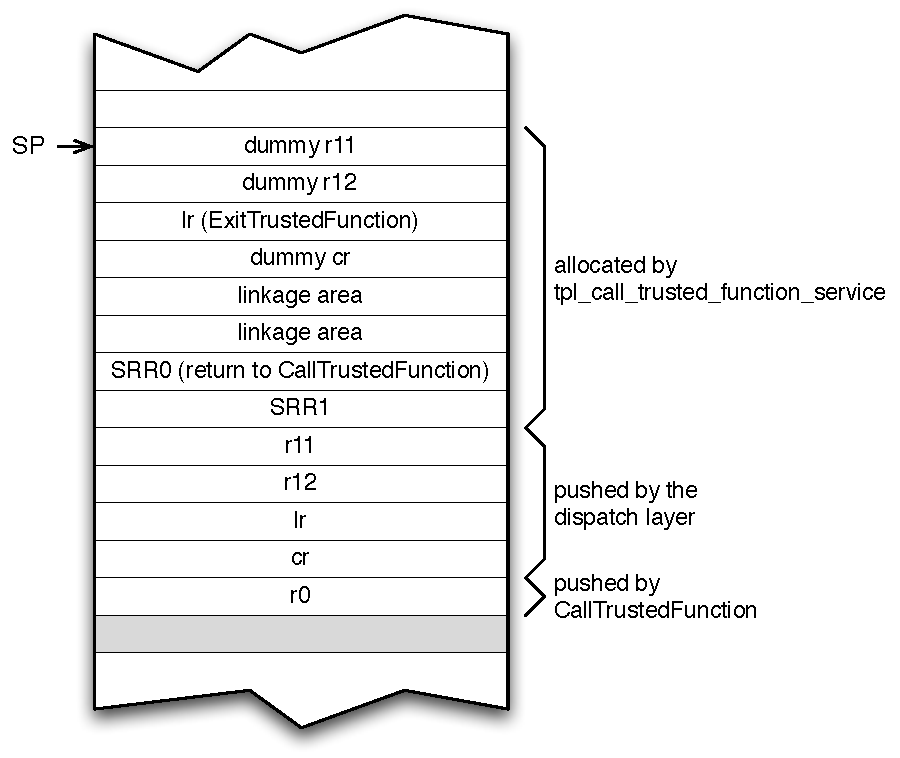
\includegraphics[scale=.6]{pictures/TFStack1} 
\end{minipage}
\begin{minipage}{0.35\textwidth}
  \caption{Process stack mapping at the end of \cfunction{tpl_call_trusted_function_service}. \reg{r0}, at the bottom of the stack has been pushed by \api{CallTrustedFunction}. \reg{cr} to \reg{r11} has been pushed by the dispatch layer. \reg{SRR0} and \reg{SRR1} are saved here by \cfunction{tpl_call_trusted_function_service} to be able to go back to the calling process. Above, the linkage area allows the trusted function to call functions. Above, a frame that will be used by the dispatch layer to restore an execution context for the trusted function is built.}\label{fig:tfstackmapping}
\end{minipage}
\end{figure}

\subsubsection{Setting the trusted function address}

The \reg{SRR0} saved by the dispatch layer after the \api{CallTrustedFunction} is changed to the address of the trusted function. This way, instead of returning to the caller, the trusted function will be executed.

\begin{lstlisting}
  lis   r11,TPL_HIG(tpl_trusted_fct_table)
  ori   r11,r11,TPL_LOW(tpl_trusted_fct_table)
  slwi  r0,r3,2
  lwzx  r12,r11,r0
  stw   r12,KS_SRR0(r1)
\end{lstlisting}

\subsubsection{Going back to the dispatch layer}

A simple \asfct{blr} goes back to the dispatch layer. The latter cleans up the process stack. Once the trusted function starts execution, the process stack is like that:

\begin{figure}[htbp] %  figure placement: here, top, bottom, or page
\begin{minipage}{0.5\textwidth}
    \centering
  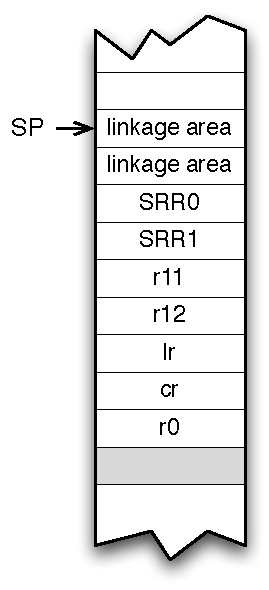
\includegraphics[scale=.6]{pictures/TFStack2} 
\end{minipage}
\begin{minipage}{0.5\textwidth}
  \caption{Process stack mapping when the trusted function starts its execution.}\label{fig:tfstackmapping2}
\end{minipage}
\end{figure}

\subsection{The ExitTrustedFunction service}\label{sec:exittfppc}

When a trusted function finishes, the context of the \api{CallTrustedFunction} must be restored to return to the caller. \api{ExitTrustedFunction} does not need to be called explicitly because its address has been set as the return address of the trusted function by \cfunction{tpl_call_trusted_function_service}. Calling \api{ExitTrustedFunction} explicitly may result in an undefined behavior or in the crash of the calling process but see below. The mapping of the process stack at start of \cfunction{tpl_exit_trusted_function_service} is shown in figure \ref{fig:ETFstack1}.

\begin{figure}[htbp] %  figure placement: here, top, bottom, or page
\begin{minipage}{0.4\textwidth}
    \centering
  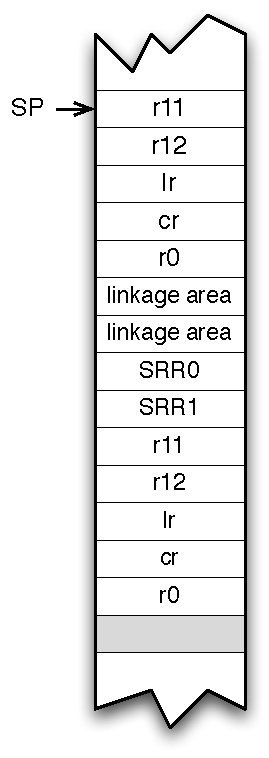
\includegraphics[scale=.6]{pictures/ETFStack1} 
\end{minipage}
\begin{minipage}{0.6\textwidth}
  \caption{Process stack mapping when the \cfunction{tpl_exit_trusted_function_service} function starts its execution.}\label{fig:ETFstack1}
\end{minipage}
\end{figure}

First, \cfunction{tpl_exit_trusted_function_service} decrements the trusted counter of the calling process. A particular attention must be given to this point because by building a fake stack frame and calling Explicitly \api{ExitTrustedFunction} to underflow this counter, a process could get a full access to the memory. So the counter is tested before to avoid to go under 0.

\begin{lstlisting}[language=C]
  lwz   r11,KS_KERN_PTR(r1) /* get the ptr to tpl_kern */
  lwz   r11,12(r11)         /* get the ptr to the runnning process desc */
  lwz   r12,4(r11)          /* get trusted_count member */
  /*
   * Warning, the trusted counter has to be check (compared to 0) to
   * avoid to decrement it if it is already 0. Without that a process
   * could build an had-hoc stack an call explicitly ExitTrustedFunction
   * to get access to all the memory.
   */
  cmpwi r12,0               /* check it is not already at 0 */
  beq   cracker_in_action   /* uh uh */
  subi  r12,r12,1           /* decrement it */
  stw   r12,4(r11)          /* put it back in the process desc */
\end{lstlisting}

\cfunction{tpl_exit_trusted_function_service} has to remove from the process stack the frame that was built by \cfunction{tpl_call_trusted_function_service}, restore \reg{SRR0} and \reg{SRR1} before returning to the dispatch layer.

\begin{lstlisting}[language=C]
cracker_in_action:
  
  /*
   * get the process stack pointer
   */
  lwz   r11,KS_SP(r1)
  
  /*
   * get back the SRR0 and SRR1
   */
  lwz   r12,PS_SRR0_OUT(r11)
  stw   r12,KS_SRR0(r1)
  lwz   r12,PS_SRR1_OUT(r11)
  stw   r12,KS_SRR1(r1)
  
  /*
   * free the process stack and update it in the kernel stack
   */
  addi  r11,r11,PS_TRUSTED_FOOTPRINT_OUT
  stw   r11,KS_SP(r1)
  
  /*
   * that's all
   */
  blr
\end{lstlisting}

\subsection{Execution of the OS Applications startup and shutdown hooks}

These hooks are executed from the kernel but with the access right of a task belonging to the OS Application. The \sysgen\ should choose one of the tasks of the OS Application to be used as context to execute the OS Application startup and shutdown hooks. Execution of an OS Application startup hook is done by the \cfunction{tpl_call_startup_hook_and_resume} function. The argument of this function is a function pointer to the hook. Similarly execution of an OS Application shutdown hook is done by the \cfunction{tpl_call_shutdown_hook_and_resume} function. These functions end by a call to \api{NextStartupHook} and \api{NextShutdownHook} services respectively to cycle through the hooks.

\subsection{The MPC5510 Memory Protection Unit}

The access control rights of the memory region descriptor rules the access of 5 bus masters (labeled from 4 to 0). Unused bus masters are set to the same access right for all the regions. Bus master 4 is used for factory testing only, so the access rights should be set to no access. Bus master 3 is the Flexray controller. Since it is not used in the current version of Trampoline, it is set to no access too. Bus master 2 is the DMA controller and for the same reason it is set to no access. Bus master 1 is the Z0 core. Again it is set to no access.

The access control rights register has the following bit usage:

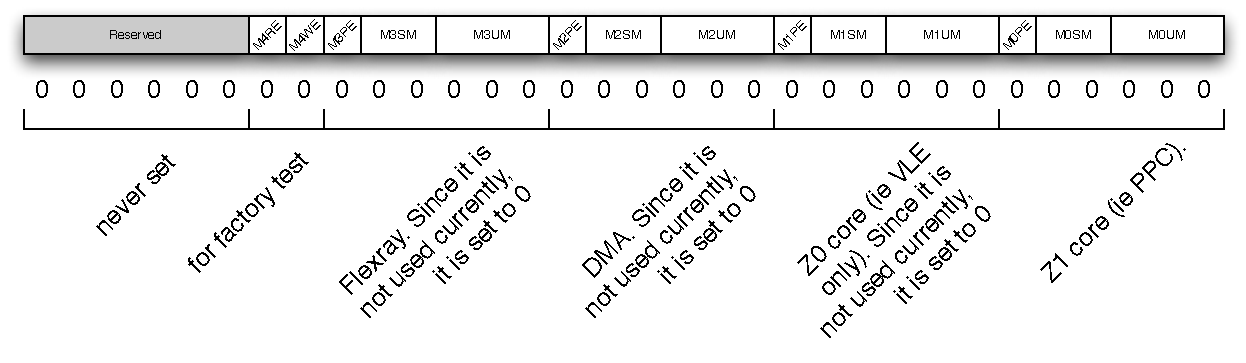
\includegraphics[width=\textwidth]{pictures/MPUacr.pdf} 

Bus master 4 is a special case. The 2 bits have the following meaning:

\rowcolors{1}{white}{light-gray}
\begin{longtable}[c]{l|p{5.15in}}
{\bf Bit}&{\bf Meaning}\\
\hline
\dreg{M4RE} & If set to 1, bus master 4 may {\bf read} memory in the region. If 0, no read is allowed\\
\dreg{M4WE} & If set to 1, bus master 4 may {\bf write} memory in the region. If 0, no write is allowed\
\end{longtable}

So in our case, these bits are set to 0.

Of course, other bus masters have more sophisticated access right:

\rowcolors{1}{white}{light-gray}
\begin{longtable}[c]{l|p{5.15in}}
{\bf Bit}&{\bf Meaning}\\
\hline
\dreg{MxPE} & The PID Enable bit. Set to 0 in our case\\
\dreg{MxSM} & These 2 bits rules the supervisor mode access control with the following meaning: $00=rwx$, $01=rx$, $10=rw$, $11=$ \textit{same as defined by \dreg{MxUM}}. In our case, it is set to $00$ for code and constants and to $11$ for data.\\
\dreg{MxUM} & These 2 bits rules the user mode access control. The first bit means $r$, the second one $w$ and the third one $x$.
\end{longtable}

Trampoline uses 4 descriptors:

\rowcolors{1}{white}{light-gray}
\begin{longtable}{l|p{1.9in}|p{2.6in}}
{\bf Descriptor} & {\bf Usage} & {\bf \dreg{MxUM} value}\\
\hline
\dreg{MPU_RGD0} & Constants and program\footnote{This region is set to the whole addressing space. This is not definitive and should be improved because reading a peripheral control register should be protected. So an additional descriptor has to be used to allow the kernel (supervisor mode) a complete access on all the memory space and no access at all for applications (user mode).}. & $rwx=00$ for supervisor mode, $rx=101$ for user mode.\\
\dreg{MPU_RGD1} & Private variables of the process. & $rw=110$ for supervisor and user mode.\\
\dreg{MPU_RGD2} & Stack of the process. & $rw=110$ for supervisor and user mode.\\
\dreg{MPU_RGD3} & Variables of the OS Application if OS Applications are used. & $rw=110$ for supervisor and user mode.\\
\end{longtable}

So values of access control bits should be:

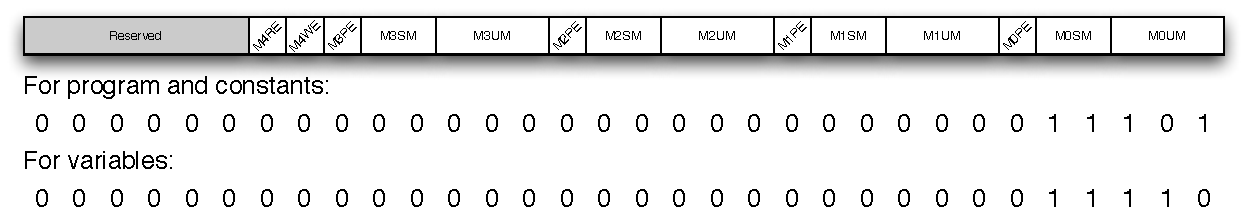
\includegraphics[width=\textwidth]{pictures/MPUprog.pdf} 

So in hexa:

\rowcolors{1}{white}{light-gray}
\begin{longtable}{l|l}
{\bf Kind} & {\bf Value}\\
\hline
Program region access & $0x00000005$\\
Variable region access & $0x0000001E$\\
\end{longtable}

\subsubsection{What happen in case of memory protection violation ?}

Two exception handler are used to handle a memory protection violation, one for data access, one for code access.

The Data Storage exception is tied to the IVOR~2 vector (VPR offset = 0x020), see page 8-2 of the {\em MPC5510 Microcontroller Family Reference Manual}.

The Instruction Storage exception is tied to the IVOR~3 vector (VPR offset = 0x030), see page 8-2 of the {\em MPC5510 Microcontroller Family Reference Manual}.

However, it appears one of these exceptions is raised when the processor is in user mode. The behavior is different in supervisor mode {\em to be completed}.

\section{ARM -- Common conventions}

\subsection{File hierarchy}

\subsection{Common definitions}

\subsection{Bootstraping}

The bootstrap must be made in specific ARM port and must call the \cfunction{main} function. If \cfunction{main} ever returns, the bootstrap code must fall into an infinite loop.

As a reason, many ARM architectures needs early specific and required initializations. This includes steps like memory mapping configuration, DRAM controller configuration, ...

Besides specific initializations, the bootstrap should :
\begin{itemize}
\item initialize stack pointer for every ARM exception modes
\item keep all external interrupts locked (will be unlocked at the first task context loading)
\item call \cfunction{main} in "system" mode (0x1F)
\end{itemize}

\subsection{Stacks}

\subsection{Interrupt management}

Kernel is not interruptible. So hardware interrupt source are disabled entering in kernel (via any case in system call, interrupt request, abort, ...).

But kernel shall be reentrant via system call (because kernel hooks can call some system calls).

\subsubsection{Interrupt and category classification}

All ARM IRQ are category 2 ISR.

All ARM FIQ are category 1 ISR.

\subsubsection{Vector table}

Each ARM exception vector points on a so called "primary" subprogram (like \cfunction{tpl\_primary\_syscall\_handler}).

To be located at address 0x00000000, this vector table is assigned to a specific section named \cfunction{.vectbl}. The linker script uses this section name to output it to address 0x00000000.

\subsubsection{System call}

\subsubsection{IRQ handling}

\subsubsection{FIQ handling}

\section{ARM -- Armadeus APF27 board}

\subsection{Debugging with Abatron BDI2000 or BDI3000 JTAG probe}

A configuration file is provided in \file{machines/arm/armadeus-apf27/bdi-config}.

To enable JTAG, if your APF27 has a FPGA, you must load the FPGA to wake it up (TO DO : explain how to do this...).

To start a debug session, follow these steps :
\begin{enumerate}
\item connects everything together
\item power up everything
\item reset the APF27 (S2 on APF27-Dev)
\item stop u-boot before it loads Linux (if MMU is started, you won't be able to load anything)
\item telnet your BDI
\item type \cfunction{reset} command in the BDI shell
\item start GDB session (\cfunction{target remote ...})
\end{enumerate}

\subsection{Configuration}

All configuration of port is done in \file{apf27\_config.h}.

\subsubsection{Stacks}

Stacks' size (stack of each exception mode) can be adjusted via the following constants. Remember that the size must be aligned to 4.

\subsubsection{CPU caches}

By default, CPU caches are disabled (for real time determinism).

\subsection{Memory mapping}

This port can be use in one of these three configurations :
\begin{enumerate}
\item No memory mapping (and thus no memory protection)
\item Memory mapping without memory protection
\item Memory mapping and memory protection
\end{enumerate}

\subsection{Memory protection}

To be written...

Some points to explain :
\begin{itemize}
\item FCSE mechanism is not used by this port (if someone is interested by this work, she's welcome)
\item address translation is not used, all VMA equals physical address
\end{itemize}

\subsubsection{MMU tables generation principle}

To be written...

Some points to explain :
\begin{itemize}
\item MMU is not disabled in privileged mode, but all useful memory areas are accessible. Thus, we hope we can find bugs easily in privіleged code.
\item useful memory areas, except processes and applications ones, are configured as accessible (read and write) in privileged mode. These memory areas are called system areas
\item some memory areas needs to be accessible by anyone (API, GCC builtin functions, common libraries, ...), they are called common areas (they are read only for unprivileged contexts)
\item there is one translation table for each process
\item all translation tables have the same system and common areas
\item there is one page table set for each process. Page tables are fine page tables. Table entries are tiny page descriptors.
\item the number of page table in a set depends on the size of the whole trampoline and application memory footprint. Then this information is given by linker via a symbol which is used by the MMU driver.
\item Page tables are accessed via a macro, as they are allocated by linker (and we cannot know the number of page tables)
\end{itemize}

\section{ARM -- Simtec EB675001 board}

\subsection{Memory map and hardware resources}

Talk about configured memory map (use of DRAM, where the bootstrap would be flashed, \ldots).

Tell which hardware resources are used by the kernel.

\subsection{Booting}

There is two way to start Trampoline on APF27 :
\begin{itemize}
\item from ELF image (in file usually called \file{trampoline})
\item from raw binary image (in file usually called \file{trampoline.bin})
\end{itemize}

\subsubsection{Booting from ELF image}

Load image with your ELF loader (the file is usually named \file{trampoline}). This can be GDB via a JTAG probe for example. Then, just start execution from \cfunction{tpl\_arm\_bootstrap\_entry} entry point. Here are commands you can type in GDB :
\begin{lstlisting}
(gdb) load
(gdb) set $pc=tpl_arm_bootstrap_entry
(gdb) break main
(gdb) continue
\end{lstlisting}

\subsubsection{Booting from raw binary image}

Load image with your binary loader to 0xA0000000 memory address. Then just start execution at this point (0xA0000000).

With u-boot, you can type these commands :
\begin{lstlisting}
BIOS> tftpboot 0xA0000000 192.168.5.20:trampoline.bin
BIOS> go 0xA0000000
\end{lstlisting}

\subsection{Internal kernel drivers}

\subsection{Hardware interrupts handling}

\subsection{Idle task}

\subsection{Exceptions handling}


\subsection{Kernel sleep service}



\part{The Goil system generator}


\printindex
\bibliographystyle{plain}
\bibliography{trampoline}

 \end{document} 